\documentclass[11pt]{article}

% The four macros of the header standard; tools/zenodo/publish_revision.py patches them when it reserves the DOI.
\newcommand{\doctype}{Preprint}
\newcommand{\docversion}{v1.00.000}
\newcommand{\docdate}{4 November 2026}
\newcommand{\versiondoi}{10.5281/zenodo.0}
\newcommand{\conceptdoi}{10.5281/zenodo.0}
\newcommand{\docidentity}{CAOS\_Contraste, the validation of the risk models of a bank}

% The packages and conventions every Contraste manuscript shares (CAOS_MANAGE conventions/manuscript-content-bar.md
% section 2). A document sets its class, the four header macros and \docidentity, then % The packages and conventions every Contraste manuscript shares (CAOS_MANAGE conventions/manuscript-content-bar.md
% section 2). A document sets its class, the four header macros and \docidentity, then % The packages and conventions every Contraste manuscript shares (CAOS_MANAGE conventions/manuscript-content-bar.md
% section 2). A document sets its class, the four header macros and \docidentity, then \input{../_shared/preamble}.
\usepackage[T1]{fontenc}
\usepackage[utf8]{inputenc}
\usepackage{lmodern}
\usepackage{microtype}
\usepackage[a4paper,margin=2.5cm]{geometry}
\usepackage{amsmath,amssymb,amsthm,mathtools,bm}
\usepackage{graphicx}
\usepackage{booktabs,longtable,tabularx,array,multirow}
\usepackage{siunitx}
\usepackage{algorithm}
\usepackage{algpseudocode}
\usepackage{caption,subcaption}
\usepackage{xcolor}
\usepackage[numbers,sort&compress]{natbib}
\usepackage[hidelinks]{hyperref}
\usepackage{cleveref}
\usepackage{orcidlink}

\sisetup{group-separator={,},group-minimum-digits=4,detect-all}
\graphicspath{{figures/}{../figures/}}
\captionsetup{font=small,labelfont=bf}
\setlength{\LTcapwidth}{\textwidth}

% Theorem environments for the Theory sections of the manuscripts.
\newtheorem{proposition}{Proposition}
\newtheorem{lemma}{Lemma}
\newtheorem{corollary}{Corollary}
\theoremstyle{definition}
\newtheorem{definition}{Definition}
\newtheorem{assumption}{Assumption}
\theoremstyle{remark}
\newtheorem{remark}{Remark}

% Notation shared by the documents (each defines it again in its notation table).
\newcommand{\E}{\mathbb{E}}
\newcommand{\Prob}{\mathbb{P}}
\newcommand{\Var}{\operatorname{Var}}
\newcommand{\Cov}{\operatorname{Cov}}
\newcommand{\VaR}{\operatorname{VaR}}
\newcommand{\ES}{\operatorname{ES}}
\newcommand{\PD}{\mathrm{PD}}
\newcommand{\LGD}{\mathrm{LGD}}
\newcommand{\EAD}{\mathrm{EAD}}
\newcommand{\ECL}{\mathrm{ECL}}
\newcommand{\indic}{\mathbf{1}}
\newcommand{\R}{\mathbb{R}}
\newcommand{\dd}{\,\mathrm{d}}

% The page-1 header block (CAOS_MANAGE conventions/manuscript-header-standard.md). The document defines \doctype,
% \docversion, \docdate, \versiondoi, \conceptdoi and \docidentity before this file; the publishing tool patches the four
% macros of the standard when it reserves the version DOI.
\newcommand{\docrepo}{github.com/fsantibanezleal/CAOS\_Contraste}
\newcommand{\headerblock}{%
\begin{center}
\fbox{\parbox{0.94\textwidth}{\small\raggedright
\textbf{\doctype} \quad$\cdot$\quad \docversion, \docdate \quad$\cdot$\quad Licence CC BY 4.0\\[2pt]
CAOS open-research programme \quad$\cdot$\quad \docidentity\\[2pt]
Version DOI \href{https://doi.org/\versiondoi}{\texttt{\versiondoi}} \quad$\cdot$\quad
concept DOI (always latest) \href{https://doi.org/\conceptdoi}{\texttt{\conceptdoi}}\\[2pt]
Not peer reviewed. Source code, data and computational records: \href{https://\docrepo}{\texttt{\docrepo}}
}}
\end{center}
\vspace{4pt}}
.
\usepackage[T1]{fontenc}
\usepackage[utf8]{inputenc}
\usepackage{lmodern}
\usepackage{microtype}
\usepackage[a4paper,margin=2.5cm]{geometry}
\usepackage{amsmath,amssymb,amsthm,mathtools,bm}
\usepackage{graphicx}
\usepackage{booktabs,longtable,tabularx,array,multirow}
\usepackage{siunitx}
\usepackage{algorithm}
\usepackage{algpseudocode}
\usepackage{caption,subcaption}
\usepackage{xcolor}
\usepackage[numbers,sort&compress]{natbib}
\usepackage[hidelinks]{hyperref}
\usepackage{cleveref}
\usepackage{orcidlink}

\sisetup{group-separator={,},group-minimum-digits=4,detect-all}
\graphicspath{{figures/}{../figures/}}
\captionsetup{font=small,labelfont=bf}
\setlength{\LTcapwidth}{\textwidth}

% Theorem environments for the Theory sections of the manuscripts.
\newtheorem{proposition}{Proposition}
\newtheorem{lemma}{Lemma}
\newtheorem{corollary}{Corollary}
\theoremstyle{definition}
\newtheorem{definition}{Definition}
\newtheorem{assumption}{Assumption}
\theoremstyle{remark}
\newtheorem{remark}{Remark}

% Notation shared by the documents (each defines it again in its notation table).
\newcommand{\E}{\mathbb{E}}
\newcommand{\Prob}{\mathbb{P}}
\newcommand{\Var}{\operatorname{Var}}
\newcommand{\Cov}{\operatorname{Cov}}
\newcommand{\VaR}{\operatorname{VaR}}
\newcommand{\ES}{\operatorname{ES}}
\newcommand{\PD}{\mathrm{PD}}
\newcommand{\LGD}{\mathrm{LGD}}
\newcommand{\EAD}{\mathrm{EAD}}
\newcommand{\ECL}{\mathrm{ECL}}
\newcommand{\indic}{\mathbf{1}}
\newcommand{\R}{\mathbb{R}}
\newcommand{\dd}{\,\mathrm{d}}

% The page-1 header block (CAOS_MANAGE conventions/manuscript-header-standard.md). The document defines \doctype,
% \docversion, \docdate, \versiondoi, \conceptdoi and \docidentity before this file; the publishing tool patches the four
% macros of the standard when it reserves the version DOI.
\newcommand{\docrepo}{github.com/fsantibanezleal/CAOS\_Contraste}
\newcommand{\headerblock}{%
\begin{center}
\fbox{\parbox{0.94\textwidth}{\small\raggedright
\textbf{\doctype} \quad$\cdot$\quad \docversion, \docdate \quad$\cdot$\quad Licence CC BY 4.0\\[2pt]
CAOS open-research programme \quad$\cdot$\quad \docidentity\\[2pt]
Version DOI \href{https://doi.org/\versiondoi}{\texttt{\versiondoi}} \quad$\cdot$\quad
concept DOI (always latest) \href{https://doi.org/\conceptdoi}{\texttt{\conceptdoi}}\\[2pt]
Not peer reviewed. Source code, data and computational records: \href{https://\docrepo}{\texttt{\docrepo}}
}}
\end{center}
\vspace{4pt}}
.
\usepackage[T1]{fontenc}
\usepackage[utf8]{inputenc}
\usepackage{lmodern}
\usepackage{microtype}
\usepackage[a4paper,margin=2.5cm]{geometry}
\usepackage{amsmath,amssymb,amsthm,mathtools,bm}
\usepackage{graphicx}
\usepackage{booktabs,longtable,tabularx,array,multirow}
\usepackage{siunitx}
\usepackage{algorithm}
\usepackage{algpseudocode}
\usepackage{caption,subcaption}
\usepackage{xcolor}
\usepackage[numbers,sort&compress]{natbib}
\usepackage[hidelinks]{hyperref}
\usepackage{cleveref}
\usepackage{orcidlink}

\sisetup{group-separator={,},group-minimum-digits=4,detect-all}
\graphicspath{{figures/}{../figures/}}
\captionsetup{font=small,labelfont=bf}
\setlength{\LTcapwidth}{\textwidth}

% Theorem environments for the Theory sections of the manuscripts.
\newtheorem{proposition}{Proposition}
\newtheorem{lemma}{Lemma}
\newtheorem{corollary}{Corollary}
\theoremstyle{definition}
\newtheorem{definition}{Definition}
\newtheorem{assumption}{Assumption}
\theoremstyle{remark}
\newtheorem{remark}{Remark}

% Notation shared by the documents (each defines it again in its notation table).
\newcommand{\E}{\mathbb{E}}
\newcommand{\Prob}{\mathbb{P}}
\newcommand{\Var}{\operatorname{Var}}
\newcommand{\Cov}{\operatorname{Cov}}
\newcommand{\VaR}{\operatorname{VaR}}
\newcommand{\ES}{\operatorname{ES}}
\newcommand{\PD}{\mathrm{PD}}
\newcommand{\LGD}{\mathrm{LGD}}
\newcommand{\EAD}{\mathrm{EAD}}
\newcommand{\ECL}{\mathrm{ECL}}
\newcommand{\indic}{\mathbf{1}}
\newcommand{\R}{\mathbb{R}}
\newcommand{\dd}{\,\mathrm{d}}

% The page-1 header block (CAOS_MANAGE conventions/manuscript-header-standard.md). The document defines \doctype,
% \docversion, \docdate, \versiondoi, \conceptdoi and \docidentity before this file; the publishing tool patches the four
% macros of the standard when it reserves the version DOI.
\newcommand{\docrepo}{github.com/fsantibanezleal/CAOS\_Contraste}
\newcommand{\headerblock}{%
\begin{center}
\fbox{\parbox{0.94\textwidth}{\small\raggedright
\textbf{\doctype} \quad$\cdot$\quad \docversion, \docdate \quad$\cdot$\quad Licence CC BY 4.0\\[2pt]
CAOS open-research programme \quad$\cdot$\quad \docidentity\\[2pt]
Version DOI \href{https://doi.org/\versiondoi}{\texttt{\versiondoi}} \quad$\cdot$\quad
concept DOI (always latest) \href{https://doi.org/\conceptdoi}{\texttt{\conceptdoi}}\\[2pt]
Not peer reviewed. Source code, data and computational records: \href{https://\docrepo}{\texttt{\docrepo}}
}}
\end{center}
\vspace{4pt}}

% Generated by tables/make_tables.py: the numbers the prose quotes. Do not edit.
\newcommand{\spLraDtwoCcc}{26.64}
\newcommand{\spLraDtwoB}{2.96}
\newcommand{\spRwDtwo}{58.0}
\newcommand{\spLraDthreeCcc}{27.58}
\newcommand{\spLraDthreeB}{3.04}
\newcommand{\spRwDthree}{58.3}
\newcommand{\spLraDfourCcc}{8.61}
\newcommand{\spLraDfourB}{1.33}
\newcommand{\spRwDfour}{47.5}
\newcommand{\spLraKeepCcc}{5.88}
\newcommand{\spLraKeepB}{1.16}
\newcommand{\spRwKeep}{45.2}
\newcommand{\fiLraDtwoCcc}{18.69}
\newcommand{\fiLraDtwoB}{1.92}
\newcommand{\fiRwDtwo}{46.9}
\newcommand{\fiLraDfourCcc}{3.65}
\newcommand{\fiLraDfourB}{0.49}
\newcommand{\fiRwDfour}{31.1}
\newcommand{\fiLraKeepCcc}{2.88}
\newcommand{\fiLraKeepB}{0.44}
\newcommand{\fiRwKeep}{30.3}
\newcommand{\moLraDtwoCcc}{11.15}
\newcommand{\moRwDtwo}{61.1}
\newcommand{\spRatioCcc}{0.322}
\newcommand{\spRatioCccLo}{0.259}
\newcommand{\spRatioCccHi}{0.391}
\newcommand{\spRatioB}{0.451}
\newcommand{\spRatioBLo}{0.370}
\newcommand{\spRatioBHi}{0.526}
\newcommand{\spRwGap}{10.5}
\newcommand{\spRwGapLo}{8.3}
\newcommand{\spRwGapHi}{13.1}
\newcommand{\spRwGapShare}{100.0}
\newcommand{\fiRatioCcc}{0.198}
\newcommand{\fiRatioCccLo}{0.133}
\newcommand{\fiRatioCccHi}{0.269}
\newcommand{\fiRatioB}{0.258}
\newcommand{\fiRatioBLo}{0.124}
\newcommand{\fiRatioBHi}{0.407}
\newcommand{\fiRwGap}{15.8}
\newcommand{\fiRwGapLo}{8.8}
\newcommand{\fiRwGapHi}{26.6}
\newcommand{\fiRwGapShare}{100.0}
\newcommand{\bootSeedRatio}{0.004}
\newcommand{\bootSeedRw}{0.7}
\newcommand{\bootB}{2{,}000}
\newcommand{\spYearsBelowB}{26}
\newcommand{\spYearsB}{26}
\newcommand{\spYearsBelowCcc}{26}
\newcommand{\spYearsCcc}{26}
\newcommand{\fiYearsBelowCcc}{22}
\newcommand{\fiYearsCcc}{24}
\newcommand{\spPooledDefDtwoCcc}{1{,}489}
\newcommand{\spPooledNDtwoCcc}{5{,}428}
\newcommand{\spPooledRateDtwoCcc}{27.43}
\newcommand{\spJeffLoDtwoCcc}{26.26}
\newcommand{\spJeffHiDtwoCcc}{28.63}
\newcommand{\spPooledDefDfourCcc}{301}
\newcommand{\spPooledNDfourCcc}{3{,}731}
\newcommand{\spPooledRateDfourCcc}{8.07}
\newcommand{\spJeffLoDfourCcc}{7.23}
\newcommand{\spJeffHiDfourCcc}{8.97}
\newcommand{\spGapYears}{18}
\newcommand{\moGapYears}{7}
\newcommand{\fiGapYears}{9}
\newcommand{\spPeakYearCccDtwo}{2009}
\newcommand{\spPeakRateCccDtwo}{50.9}
\newcommand{\spPeakYearCccDfour}{2009}
\newcommand{\spPeakRateCccDfour}{23.9}
\newcommand{\agencyRatio}{2.4}
\newcommand{\spWdShareAll}{7.9}
\newcommand{\spWdShareB}{12.3}
\newcommand{\spWdShareCcc}{28.5}
\newcommand{\spWdShareAaa}{2.8}
\newcommand{\spCohorts}{26}
\newcommand{\spMeanCohort}{7111}
\newcommand{\moCohorts}{26}
\newcommand{\moMeanCohort}{3758}
\newcommand{\fiCohorts}{24}
\newcommand{\fiMeanCohort}{2857}
\newcommand{\repsNew}{1{,}000}
\newcommand{\minWd}{5}
\newcommand{\minTheory}{1}
\newcommand{\repsCommitted}{200}
\newcommand{\repsTests}{1{,}000}
\newcommand{\truthB}{1.17}
\newcommand{\truthCcc}{8.06}
\newcommand{\rwTruth}{46.8}
\newcommand{\reproMax}{5\times10^{-11}}
\newcommand{\removedBkZero}{2.6}
\newcommand{\removedBkZerose}{0.4}
\newcommand{\removedCcckZero}{2.6}
\newcommand{\removedCcckZerose}{0.3}
\newcommand{\removedYoneBbbkZero}{2.0}
\newcommand{\removedYoneBbbkZerose}{2.8}
\newcommand{\removedYoneBbkZero}{2.8}
\newcommand{\removedYoneBbkZerose}{1.7}
\newcommand{\removedYoneBkZero}{1.0}
\newcommand{\removedYoneBkZerose}{0.8}
\newcommand{\removedYoneCcckZero}{1.5}
\newcommand{\removedYoneCcckZerose}{0.8}
\newcommand{\rwremovedkZero}{0.38}
\newcommand{\rwremovedkZerose}{0.06}
\newcommand{\rwAbsremovedkZero}{0.38}
\newcommand{\keptBkZero}{-3.4}
\newcommand{\keptBkZerose}{0.4}
\newcommand{\keptCcckZero}{-3.1}
\newcommand{\keptCcckZerose}{0.3}
\newcommand{\keptYoneBbbkZero}{-4.0}
\newcommand{\keptYoneBbbkZerose}{2.6}
\newcommand{\keptYoneBbkZero}{-3.2}
\newcommand{\keptYoneBbkZerose}{1.6}
\newcommand{\keptYoneBkZero}{-4.9}
\newcommand{\keptYoneBkZerose}{0.8}
\newcommand{\keptYoneCcckZero}{-4.2}
\newcommand{\keptYoneCcckZerose}{0.8}
\newcommand{\rwkeptkZero}{-0.60}
\newcommand{\rwkeptkZerose}{0.06}
\newcommand{\rwAbskeptkZero}{0.60}
\newcommand{\followedBkZero}{-0.2}
\newcommand{\followedBkZerose}{0.4}
\newcommand{\followedCcckZero}{-0.3}
\newcommand{\followedCcckZerose}{0.3}
\newcommand{\followedYoneBbbkZero}{-0.4}
\newcommand{\followedYoneBbbkZerose}{2.7}
\newcommand{\followedYoneBbkZero}{0.3}
\newcommand{\followedYoneBbkZerose}{1.6}
\newcommand{\followedYoneBkZero}{-1.8}
\newcommand{\followedYoneBkZerose}{0.8}
\newcommand{\followedYoneCcckZero}{-1.6}
\newcommand{\followedYoneCcckZerose}{0.8}
\newcommand{\rwfollowedkZero}{-0.09}
\newcommand{\rwfollowedkZerose}{0.06}
\newcommand{\rwAbsfollowedkZero}{0.09}
\newcommand{\latentBkZero}{-0.2}
\newcommand{\latentBkZerose}{0.4}
\newcommand{\latentCcckZero}{-0.3}
\newcommand{\latentCcckZerose}{0.3}
\newcommand{\latentYoneBbbkZero}{-0.4}
\newcommand{\latentYoneBbbkZerose}{2.7}
\newcommand{\latentYoneBbkZero}{0.3}
\newcommand{\latentYoneBbkZerose}{1.6}
\newcommand{\latentYoneBkZero}{-1.8}
\newcommand{\latentYoneBkZerose}{0.8}
\newcommand{\latentYoneCcckZero}{-1.6}
\newcommand{\latentYoneCcckZerose}{0.8}
\newcommand{\rwlatentkZero}{-0.08}
\newcommand{\rwlatentkZerose}{0.06}
\newcommand{\rwAbslatentkZero}{0.08}
\newcommand{\removedBkOne}{-2.7}
\newcommand{\removedBkOnese}{0.4}
\newcommand{\removedCcckOne}{-1.7}
\newcommand{\removedCcckOnese}{0.3}
\newcommand{\removedYoneBbbkOne}{0.5}
\newcommand{\removedYoneBbbkOnese}{2.7}
\newcommand{\removedYoneBbkOne}{0.1}
\newcommand{\removedYoneBbkOnese}{1.7}
\newcommand{\removedYoneBkOne}{-1.6}
\newcommand{\removedYoneBkOnese}{0.8}
\newcommand{\removedYoneCcckOne}{0.2}
\newcommand{\removedYoneCcckOnese}{0.8}
\newcommand{\rwremovedkOne}{-0.42}
\newcommand{\rwremovedkOnese}{0.06}
\newcommand{\rwAbsremovedkOne}{0.42}
\newcommand{\keptBkOne}{-8.5}
\newcommand{\keptBkOnese}{0.4}
\newcommand{\keptCcckOne}{-7.5}
\newcommand{\keptCcckOnese}{0.3}
\newcommand{\keptYoneBbbkOne}{-5.4}
\newcommand{\keptYoneBbbkOnese}{2.5}
\newcommand{\keptYoneBbkOne}{-5.7}
\newcommand{\keptYoneBbkOnese}{1.6}
\newcommand{\keptYoneBkOne}{-7.4}
\newcommand{\keptYoneBkOnese}{0.8}
\newcommand{\keptYoneCcckOne}{-5.9}
\newcommand{\keptYoneCcckOnese}{0.8}
\newcommand{\rwkeptkOne}{-1.40}
\newcommand{\rwkeptkOnese}{0.06}
\newcommand{\rwAbskeptkOne}{1.40}
\newcommand{\followedBkOne}{-2.3}
\newcommand{\followedBkOnese}{0.4}
\newcommand{\followedCcckOne}{-2.1}
\newcommand{\followedCcckOnese}{0.3}
\newcommand{\followedYoneBbbkOne}{1.0}
\newcommand{\followedYoneBbbkOnese}{2.5}
\newcommand{\followedYoneBbkOne}{0.3}
\newcommand{\followedYoneBbkOnese}{1.6}
\newcommand{\followedYoneBkOne}{-1.1}
\newcommand{\followedYoneBkOnese}{0.8}
\newcommand{\followedYoneCcckOne}{-0.5}
\newcommand{\followedYoneCcckOnese}{0.8}
\newcommand{\rwfollowedkOne}{-0.37}
\newcommand{\rwfollowedkOnese}{0.06}
\newcommand{\rwAbsfollowedkOne}{0.37}
\newcommand{\latentBkOne}{-0.2}
\newcommand{\latentBkOnese}{0.4}
\newcommand{\latentCcckOne}{0.3}
\newcommand{\latentCcckOnese}{0.3}
\newcommand{\latentYoneBbbkOne}{1.0}
\newcommand{\latentYoneBbbkOnese}{2.5}
\newcommand{\latentYoneBbkOne}{0.3}
\newcommand{\latentYoneBbkOnese}{1.6}
\newcommand{\latentYoneBkOne}{-1.1}
\newcommand{\latentYoneBkOnese}{0.8}
\newcommand{\latentYoneCcckOne}{-0.5}
\newcommand{\latentYoneCcckOnese}{0.8}
\newcommand{\rwlatentkOne}{0.02}
\newcommand{\rwlatentkOnese}{0.06}
\newcommand{\rwAbslatentkOne}{0.02}
\newcommand{\removedBkThree}{-12.0}
\newcommand{\removedBkThreese}{0.4}
\newcommand{\removedCcckThree}{-11.2}
\newcommand{\removedCcckThreese}{0.3}
\newcommand{\removedYoneBbbkThree}{-6.6}
\newcommand{\removedYoneBbbkThreese}{2.7}
\newcommand{\removedYoneBbkThree}{-8.0}
\newcommand{\removedYoneBbkThreese}{1.6}
\newcommand{\removedYoneBkThree}{-6.6}
\newcommand{\removedYoneBkThreese}{0.7}
\newcommand{\removedYoneCcckThree}{-4.7}
\newcommand{\removedYoneCcckThreese}{0.8}
\newcommand{\rwremovedkThree}{-2.12}
\newcommand{\rwremovedkThreese}{0.06}
\newcommand{\rwAbsremovedkThree}{2.12}
\newcommand{\keptBkThree}{-17.3}
\newcommand{\keptBkThreese}{0.3}
\newcommand{\keptCcckThree}{-17.1}
\newcommand{\keptCcckThreese}{0.3}
\newcommand{\keptYoneBbbkThree}{-12.1}
\newcommand{\keptYoneBbbkThreese}{2.5}
\newcommand{\keptYoneBbkThree}{-13.4}
\newcommand{\keptYoneBbkThreese}{1.6}
\newcommand{\keptYoneBkThree}{-12.2}
\newcommand{\keptYoneBkThreese}{0.7}
\newcommand{\keptYoneCcckThree}{-11.1}
\newcommand{\keptYoneCcckThreese}{0.7}
\newcommand{\rwkeptkThree}{-3.07}
\newcommand{\rwkeptkThreese}{0.06}
\newcommand{\rwAbskeptkThree}{3.07}
\newcommand{\followedBkThree}{-6.1}
\newcommand{\followedBkThreese}{0.4}
\newcommand{\followedCcckThree}{-7.0}
\newcommand{\followedCcckThreese}{0.3}
\newcommand{\followedYoneBbbkThree}{-1.2}
\newcommand{\followedYoneBbbkThreese}{2.7}
\newcommand{\followedYoneBbkThree}{-2.5}
\newcommand{\followedYoneBbkThreese}{1.6}
\newcommand{\followedYoneBkThree}{-0.4}
\newcommand{\followedYoneBkThreese}{0.8}
\newcommand{\followedYoneCcckThree}{-0.6}
\newcommand{\followedYoneCcckThreese}{0.8}
\newcommand{\rwfollowedkThree}{-1.15}
\newcommand{\rwfollowedkThreese}{0.06}
\newcommand{\rwAbsfollowedkThree}{1.15}
\newcommand{\latentBkThree}{-0.3}
\newcommand{\latentBkThreese}{0.3}
\newcommand{\latentCcckThree}{-0.3}
\newcommand{\latentCcckThreese}{0.3}
\newcommand{\latentYoneBbbkThree}{-1.2}
\newcommand{\latentYoneBbbkThreese}{2.7}
\newcommand{\latentYoneBbkThree}{-2.5}
\newcommand{\latentYoneBbkThreese}{1.6}
\newcommand{\latentYoneBkThree}{-0.4}
\newcommand{\latentYoneBkThreese}{0.8}
\newcommand{\latentYoneCcckThree}{-0.6}
\newcommand{\latentYoneCcckThreese}{0.8}
\newcommand{\rwlatentkThree}{-0.11}
\newcommand{\rwlatentkThreese}{0.06}
\newcommand{\rwAbslatentkThree}{0.11}
\newcommand{\removedBkNine}{-35.1}
\newcommand{\removedBkNinese}{0.3}
\newcommand{\removedCcckNine}{-34.3}
\newcommand{\removedCcckNinese}{0.3}
\newcommand{\removedYoneBbbkNine}{-18.9}
\newcommand{\removedYoneBbbkNinese}{2.5}
\newcommand{\removedYoneBbkNine}{-21.9}
\newcommand{\removedYoneBbkNinese}{1.5}
\newcommand{\removedYoneBkNine}{-20.9}
\newcommand{\removedYoneBkNinese}{0.7}
\newcommand{\removedYoneCcckNine}{-18.1}
\newcommand{\removedYoneCcckNinese}{0.7}
\newcommand{\rwremovedkNine}{-6.54}
\newcommand{\rwremovedkNinese}{0.06}
\newcommand{\rwAbsremovedkNine}{6.54}
\newcommand{\keptBkNine}{-39.2}
\newcommand{\keptBkNinese}{0.3}
\newcommand{\keptCcckNine}{-39.7}
\newcommand{\keptCcckNinese}{0.3}
\newcommand{\keptYoneBbbkNine}{-23.7}
\newcommand{\keptYoneBbbkNinese}{2.3}
\newcommand{\keptYoneBbkNine}{-26.6}
\newcommand{\keptYoneBbkNinese}{1.4}
\newcommand{\keptYoneBkNine}{-25.9}
\newcommand{\keptYoneBkNinese}{0.7}
\newcommand{\keptYoneCcckNine}{-25.2}
\newcommand{\keptYoneCcckNinese}{0.7}
\newcommand{\rwkeptkNine}{-7.43}
\newcommand{\rwkeptkNinese}{0.06}
\newcommand{\rwAbskeptkNine}{7.43}
\newcommand{\followedBkNine}{-15.6}
\newcommand{\followedBkNinese}{0.3}
\newcommand{\followedCcckNine}{-19.0}
\newcommand{\followedCcckNinese}{0.3}
\newcommand{\followedYoneBbbkNine}{-1.1}
\newcommand{\followedYoneBbbkNinese}{2.6}
\newcommand{\followedYoneBbkNine}{0.1}
\newcommand{\followedYoneBbkNinese}{1.7}
\newcommand{\followedYoneBkNine}{1.4}
\newcommand{\followedYoneBkNinese}{0.8}
\newcommand{\followedYoneCcckNine}{-0.9}
\newcommand{\followedYoneCcckNinese}{0.8}
\newcommand{\rwfollowedkNine}{-2.94}
\newcommand{\rwfollowedkNinese}{0.06}
\newcommand{\rwAbsfollowedkNine}{2.94}
\newcommand{\latentBkNine}{0.3}
\newcommand{\latentBkNinese}{0.4}
\newcommand{\latentCcckNine}{-0.5}
\newcommand{\latentCcckNinese}{0.3}
\newcommand{\latentYoneBbbkNine}{-1.1}
\newcommand{\latentYoneBbbkNinese}{2.6}
\newcommand{\latentYoneBbkNine}{0.1}
\newcommand{\latentYoneBbkNinese}{1.7}
\newcommand{\latentYoneBkNine}{1.4}
\newcommand{\latentYoneBkNinese}{0.8}
\newcommand{\latentYoneCcckNine}{-0.9}
\newcommand{\latentYoneCcckNinese}{0.8}
\newcommand{\rwlatentkNine}{-0.11}
\newcommand{\rwlatentkNinese}{0.06}
\newcommand{\rwAbslatentkNine}{0.11}
\newcommand{\removedBkNineteen}{-60.3}
\newcommand{\removedBkNineteense}{0.3}
\newcommand{\removedCcckNineteen}{-58.9}
\newcommand{\removedCcckNineteense}{0.2}
\newcommand{\removedYoneBbbkNineteen}{-38.2}
\newcommand{\removedYoneBbbkNineteense}{2.1}
\newcommand{\removedYoneBbkNineteen}{-38.2}
\newcommand{\removedYoneBbkNineteense}{1.4}
\newcommand{\removedYoneBkNineteen}{-39.4}
\newcommand{\removedYoneBkNineteense}{0.6}
\newcommand{\removedYoneCcckNineteen}{-34.0}
\newcommand{\removedYoneCcckNineteense}{0.7}
\newcommand{\rwremovedkNineteen}{-12.24}
\newcommand{\rwremovedkNineteense}{0.06}
\newcommand{\rwAbsremovedkNineteen}{12.24}
\newcommand{\keptBkNineteen}{-62.9}
\newcommand{\keptBkNineteense}{0.2}
\newcommand{\keptCcckNineteen}{-62.9}
\newcommand{\keptCcckNineteense}{0.2}
\newcommand{\keptYoneBbbkNineteen}{-41.8}
\newcommand{\keptYoneBbbkNineteense}{2.0}
\newcommand{\keptYoneBbkNineteen}{-42.0}
\newcommand{\keptYoneBbkNineteense}{1.3}
\newcommand{\keptYoneBkNineteen}{-43.6}
\newcommand{\keptYoneBkNineteense}{0.6}
\newcommand{\keptYoneCcckNineteen}{-41.2}
\newcommand{\keptYoneCcckNineteense}{0.6}
\newcommand{\rwkeptkNineteen}{-12.98}
\newcommand{\rwkeptkNineteense}{0.06}
\newcommand{\rwAbskeptkNineteen}{12.98}
\newcommand{\followedBkNineteen}{-28.6}
\newcommand{\followedBkNineteense}{0.3}
\newcommand{\followedCcckNineteen}{-33.0}
\newcommand{\followedCcckNineteense}{0.3}
\newcommand{\followedYoneBbbkNineteen}{1.9}
\newcommand{\followedYoneBbbkNineteense}{2.6}
\newcommand{\followedYoneBbkNineteen}{-0.6}
\newcommand{\followedYoneBbkNineteense}{1.7}
\newcommand{\followedYoneBkNineteen}{0.1}
\newcommand{\followedYoneBkNineteense}{0.8}
\newcommand{\followedYoneCcckNineteen}{-1.5}
\newcommand{\followedYoneCcckNineteense}{0.8}
\newcommand{\rwfollowedkNineteen}{-5.35}
\newcommand{\rwfollowedkNineteense}{0.06}
\newcommand{\rwAbsfollowedkNineteen}{5.35}
\newcommand{\latentBkNineteen}{0.2}
\newcommand{\latentBkNineteense}{0.4}
\newcommand{\latentCcckNineteen}{-0.1}
\newcommand{\latentCcckNineteense}{0.3}
\newcommand{\latentYoneBbbkNineteen}{1.9}
\newcommand{\latentYoneBbbkNineteense}{2.6}
\newcommand{\latentYoneBbkNineteen}{-0.6}
\newcommand{\latentYoneBbkNineteense}{1.7}
\newcommand{\latentYoneBkNineteen}{0.1}
\newcommand{\latentYoneBkNineteense}{0.8}
\newcommand{\latentYoneCcckNineteen}{-1.5}
\newcommand{\latentYoneCcckNineteense}{0.8}
\newcommand{\rwlatentkNineteen}{0.01}
\newcommand{\rwlatentkNineteense}{0.06}
\newcommand{\rwAbslatentkNineteen}{0.01}
\newcommand{\latentRwMaxZ}{2.2}
\newcommand{\committedremovedkNine}{-34}
\newcommand{\committedremovedkZero}{2}
\newcommand{\committedkeptkNine}{-38}
\newcommand{\committedkeptkZero}{-4}
\newcommand{\committedfollowedkNine}{-15}
\newcommand{\committedfollowedkZero}{-0}
\newcommand{\committedremovedkZeroPrec}{2.4}
\newcommand{\seRemovedPaired}{3.0}
\newcommand{\seRemovedUnpaired}{5.6}
\newcommand{\seRatio}{1.88}
\newcommand{\seRatioPct}{47}
\newcommand{\testthkZerofive}{2.8}
\newcommand{\testthkZerofivelo}{1.9}
\newcommand{\testthkZerofivehi}{4.0}
\newcommand{\testthkZeroone}{0.4}
\newcommand{\testthkZeroonelo}{0.2}
\newcommand{\testthkZeroonehi}{1.0}
\newcommand{\testmrkZerofive}{0.2}
\newcommand{\testmrkZerofivelo}{0.1}
\newcommand{\testmrkZerofivehi}{0.7}
\newcommand{\testmrkZeroone}{0.0}
\newcommand{\testmrkZeroonelo}{0.0}
\newcommand{\testmrkZeroonehi}{0.4}
\newcommand{\testthkNinefive}{5.8}
\newcommand{\testthkNinefivelo}{4.5}
\newcommand{\testthkNinefivehi}{7.4}
\newcommand{\testthkNineone}{1.0}
\newcommand{\testthkNineonelo}{0.5}
\newcommand{\testthkNineonehi}{1.8}
\newcommand{\testmrkNinefive}{1.4}
\newcommand{\testmrkNinefivelo}{0.8}
\newcommand{\testmrkNinefivehi}{2.3}
\newcommand{\testmrkNineone}{0.0}
\newcommand{\testmrkNineonelo}{0.0}
\newcommand{\testmrkNineonehi}{0.4}
\newcommand{\testthkNineteenfive}{8.8}
\newcommand{\testthkNineteenfivelo}{7.2}
\newcommand{\testthkNineteenfivehi}{10.7}
\newcommand{\testthkNineteenone}{2.1}
\newcommand{\testthkNineteenonelo}{1.4}
\newcommand{\testthkNineteenonehi}{3.2}
\newcommand{\testmrkNineteenfive}{16.3}
\newcommand{\testmrkNineteenfivelo}{14.1}
\newcommand{\testmrkNineteenfivehi}{18.7}
\newcommand{\testmrkNineteenone}{4.3}
\newcommand{\testmrkNineteenonelo}{3.2}
\newcommand{\testmrkNineteenonehi}{5.7}
\newcommand{\zeroAaaRemoved}{99}
\newcommand{\thMaxZ}{1.69}
\newcommand{\thNcmp}{80}
\newcommand{\thRepsB}{40}
\newcommand{\thObligB}{100{,}000}
\newcommand{\thObligC}{50{,}000}
\newcommand{\thLambdaB}{0.01180}
\newcommand{\thBremovedPoolkZero}{3.0}
\newcommand{\thBkeptPoolkZero}{-2.9}
\newcommand{\thBfollowedPoolkZero}{-0.0}
\newcommand{\thBremovedYonekZero}{3.0}
\newcommand{\thBkeptYonekZero}{-2.9}
\newcommand{\thBfollowedYonekZero}{-0.0}
\newcommand{\thBremovedPoolkOne}{-2.2}
\newcommand{\thBkeptPoolkOne}{-7.9}
\newcommand{\thBfollowedPoolkOne}{-2.2}
\newcommand{\thBremovedYonekOne}{0.1}
\newcommand{\thBkeptYonekOne}{-5.8}
\newcommand{\thBfollowedYonekOne}{-0.0}
\newcommand{\thBremovedPoolkThree}{-11.8}
\newcommand{\thBkeptPoolkThree}{-17.1}
\newcommand{\thBfollowedPoolkThree}{-6.5}
\newcommand{\thBremovedYonekThree}{-5.4}
\newcommand{\thBkeptYonekThree}{-11.1}
\newcommand{\thBfollowedYonekThree}{-0.0}
\newcommand{\thBremovedPoolkNine}{-35.0}
\newcommand{\thBkeptPoolkNine}{-39.0}
\newcommand{\thBfollowedPoolkNine}{-17.4}
\newcommand{\thBremovedYonekNine}{-19.7}
\newcommand{\thBkeptYonekNine}{-24.8}
\newcommand{\thBfollowedYonekNine}{-0.0}
\newcommand{\thBremovedPoolkNineteen}{-60.0}
\newcommand{\thBkeptPoolkNineteen}{-62.6}
\newcommand{\thBfollowedPoolkNineteen}{-30.9}
\newcommand{\thBremovedYonekNineteen}{-37.5}
\newcommand{\thBkeptYonekNineteen}{-41.7}
\newcommand{\thBfollowedYonekNineteen}{-0.0}
\newcommand{\thCccremovedPoolkZero}{2.8}
\newcommand{\thCcckeptPoolkZero}{-2.9}
\newcommand{\thCccfollowedPoolkZero}{0.0}
\newcommand{\thCccremovedYonekZero}{2.8}
\newcommand{\thCcckeptYonekZero}{-2.9}
\newcommand{\thCccfollowedYonekZero}{0.0}
\newcommand{\thCccremovedPoolkOne}{-1.8}
\newcommand{\thCcckeptPoolkOne}{-7.6}
\newcommand{\thCccfollowedPoolkOne}{-2.0}
\newcommand{\thCccremovedYonekOne}{0.4}
\newcommand{\thCcckeptYonekOne}{-5.7}
\newcommand{\thCccfollowedYonekOne}{0.0}
\newcommand{\thCccremovedPoolkThree}{-10.3}
\newcommand{\thCcckeptPoolkThree}{-16.4}
\newcommand{\thCccfollowedPoolkThree}{-5.9}
\newcommand{\thCccremovedYonekThree}{-4.4}
\newcommand{\thCcckeptYonekThree}{-10.9}
\newcommand{\thCccfollowedYonekThree}{0.0}
\newcommand{\thCccremovedPoolkNine}{-31.8}
\newcommand{\thCcckeptPoolkNine}{-37.6}
\newcommand{\thCccfollowedPoolkNine}{-15.9}
\newcommand{\thCccremovedYonekNine}{-17.1}
\newcommand{\thCcckeptYonekNine}{-24.5}
\newcommand{\thCccfollowedYonekNine}{0.0}
\newcommand{\thCccremovedPoolkNineteen}{-56.1}
\newcommand{\thCcckeptPoolkNineteen}{-60.8}
\newcommand{\thCccfollowedPoolkNineteen}{-28.4}
\newcommand{\thCccremovedYonekNineteen}{-33.6}
\newcommand{\thCcckeptYonekNineteen}{-41.3}
\newcommand{\thCccfollowedYonekNineteen}{0.0}
\newcommand{\foRemkZero}{3.1}
\newcommand{\foKeptkZero}{-2.9}
\newcommand{\foFolkZero}{0.0}
\newcommand{\foRemkOne}{0.1}
\newcommand{\foKeptkOne}{-5.8}
\newcommand{\foFolkOne}{-2.9}
\newcommand{\foRemkTwo}{-2.8}
\newcommand{\foKeptkTwo}{-8.5}
\newcommand{\foFolkTwo}{-5.8}
\newcommand{\foRemkThree}{-5.6}
\newcommand{\foKeptkThree}{-11.1}
\newcommand{\foFolkThree}{-8.5}
\newcommand{\foRemkFive}{-10.8}
\newcommand{\foKeptkFive}{-16.0}
\newcommand{\foFolkFive}{-13.6}
\newcommand{\foRemkNine}{-20.2}
\newcommand{\foKeptkNine}{-24.8}
\newcommand{\foFolkNine}{-22.7}
\newcommand{\foRemkNineteen}{-38.2}
\newcommand{\foKeptkNineteen}{-41.8}
\newcommand{\foFolkNineteen}{-40.3}
\newcommand{\genSizes}{75, 822, 1{,}814, 1{,}756, 1{,}054, 1{,}391, 201}
\newcommand{\wRate}{6}
\newcommand{\limKeptKone}{100}
\newcommand{\waldAaaFifty}{0.33}
\newcommand{\waldAaaFiftyFour}{0.3278}
\newcommand{\acAaaFifty}{100.00}
\newcommand{\jeffAaaFifty}{99.67}
\newcommand{\waldAaFifty}{0.2}
\newcommand{\jeffAaaThou}{93.6}
\newcommand{\jeffBbThou}{94.4}
\newcommand{\waldAaaGen}{0.5}
\newcommand{\waldAaGen}{4.0}
\newcommand{\waldAGen}{41}
\newcommand{\waldBbbFifty}{4.0}
\newcommand{\waldBFifty}{44.5}
\newcommand{\waldCccFifty}{91.4}
\newcommand{\jeffMinFifty}{96.0}
\newcommand{\acMinFifty}{95.5}
\newcommand{\waldAaaThou}{6.4}
\newcommand{\waldAaTwoHundred}{0.98}
\newcommand{\pAaa}{0.0066}
\newcommand{\pB}{1.173}
\newcommand{\pCcc}{8.06}
\newcommand{\cfAaaFifty}{0.3278}
\newcommand{\cfAaaFiftyDiff}{4.3\times10^{-12}}
\newcommand{\cfJeffMaxDiff}{7.0\times10^{-15}}
\newcommand{\lenWaldAaaFifty}{1.9}
\newcommand{\lenJeffAaaFifty}{489}
\newcommand{\lenAcAaaFifty}{853}
\newcommand{\pAaaBp}{0.66}
\newcommand{\overlapAaaAaThou}{1.00}
\newcommand{\overlapBCccTwo}{0.21}
\newcommand{\waldFirstBb}{2{,}000}
\newcommand{\waldFirstCcc}{50}
\newcommand{\waldFirstAaa}{none within the grid}
\newcommand{\waldAaaFiftyK}{83.7}
\newcommand{\gridMax}{50{,}000}
\newcommand{\repsNeeded}{30{,}400}

\makeatletter
\def\input@path{{sections/}}
\makeatother

% Notation of this manuscript.
\newcommand{\Dtwo}{\mathrm{D2}}
\newcommand{\Dthree}{\mathrm{D3}}
\newcommand{\Dfour}{\mathrm{D4}}
\newcommand{\Dkeep}{\mathrm{K}}
\newcommand{\RW}{\mathrm{RW}}

\title{The default definition as part of the PD: informative withdrawals and thin grades}
\author{Felipe Santib\'a\~nez-Leal~\orcidlink{0000-0002-0150-3246}\\
\small CAOS open-research programme, Santiago, Chile\\
\small \texttt{fsantibanez@gmail.com}}
\date{\docdate}

\begin{document}
\maketitle
\headerblock

\begin{abstract}
A bank that sets the PD of a grade from the published statistics of rating agencies inherits two choices it seldom shows: which events count as a default, and what becomes of a rating withdrawn during the year. Estimators take the published tables as given, and the European repository that publishes them sets no common definition of a default event. We propose a measurement protocol that treats the definition and the treatment of withdrawals as parameters of the PD: the PD of every grade under each page of the repository with its capital, the bias of each treatment of withdrawn ratings on rating paths of known truth, matrix-test rejection rates, and the exact coverage of interval estimators. On S\&P's corporate cohorts of 2000 to 2025 the long-run PD of CCC to C is $\spLraDtwoCcc\%$ on the default page and $\spLraDfourCcc\%$ on the transition page, and the IRB risk weight of the cohort mix falls from $\spRwDtwo\%$ to $\spRwDfour\%$. With withdrawal ten times as likely in the year before default, removing the withdrawn ratings understates the PD of grade B by $\removedBkNine\pm\removedBkNinese$ percent and following them to the year end by $\followedBkNine\pm\followedBkNinese$ percent, while two matrix tests reject in $\testthkNinefive\%$ and $\testmrkNinefive\%$ of repetitions at the 5\% level. Closed forms for the bias of each treatment agree with the simulation within $\thMaxZ$ standard errors. With 50 obligors per grade the Wald interval contains the PD of AAA in $\waldAaaFifty\%$ of samples. The protocol measures these biases and repairs none.

\end{abstract}

\section{Introduction}
\label{sec:introduction}
A bank that validates an internal rating system meets rating agencies' statistics wherever its own default history is short. The background to the guidelines of the European Banking Authority on PD estimation describes an approach in which an institution uses migration matrices ``for the purpose of estimating long-run average default rates covering the full historical observation period''; the guidelines define the long-run average as the observed average of the one-year default rates (paragraph 84) and ask that an obligor whose obligation is closed during the year stay in the denominator of the one-year default rate (paragraphs 73 and 76) \citep{EBA_2017}. The statistics a validator can reach for that purpose are those of ESMA's central repository, CEREP, which publishes aggregated counts for the registered agencies \citep{ESMA_CEREP}. CEREP counts defaults on three pages, and each page counts differently. The default page divides the distinct ratings that defaulted by the ratings of the initial cohort whether or not they were withdrawn afterwards; the defaults page counts every default event of the initial cohort; and the transition page reports the ratings in a default category at the end of the period over the cohort less its withdrawals, so that a rating withdrawn by the end of the period leaves the sample whatever happened to it before. ESMA states that, for the purposes of CEREP, no deterministic definition of a default event has been set, so that the definitions might differ between agencies. % voice-ok: withdrawn rating, the domain term of the study

The choice among the pages is not a detail. On the corporate cohorts of S\&P for 2000 to 2025 the long-run average PD of the grade CCC to C is $\spLraDtwoCcc\%$ read from the default page and $\spLraDfourCcc\%$ read from the transition page, and the IRB risk weight of the cohort mix, computed with the Basel III function, moves from $\spRwDtwo\%$ to $\spRwDfour\%$. A model owner who reports ``the PD of the grade'' without naming the page reports a number that can differ by a factor of three from the one a colleague reads on the neighbouring page. The data cannot say which page is right, because the pages answer different questions; what a validator can do is to name the definition with every PD and to measure how far the others are.

Two further choices sit behind the transition page and every estimator built on it. The first is the treatment of withdrawn ratings. The method that Schuermann and Hanson describe as the industry standard removes a withdrawn rating from the sample and so treats withdrawal as uninformative about default \citep{Schuermann_2004}; the guidelines' paragraph 76 asks that closed obligations remain in the denominator. If withdrawals are more likely shortly before a default (an issuer in distress may stop cooperating with its agency), then each treatment is biased by an amount that the data alone cannot reveal, because a withdrawn rating that would have defaulted is never seen to default \citep{Cantor_2007,Tsiatis_1975}. The second choice is how many obligors a grade holds. The investment grades of a cohort hold few defaults: the PD of AAA in the generator we use is $\pAaaBp$ basis points, so that a cohort of 50 obligors almost never contains a default, and an interval built on the observed rate collapses to a point exactly when the information is thinnest \citep{Brown_2001,Hanson_2006}. % voice-ok: withdrawn rating, the domain term of the study

We propose a measurement protocol that turns these three choices into measured quantities. The protocol reads the PD of every grade under each page and carries the difference to capital through the IRB risk-weight function; it generates rating paths from a generator whose PDs are known, withdraws ratings at a rate that rises by the factor $1+k$ in the year before default, and measures the bias of each treatment of withdrawals along a ladder of $k$; it runs the standard matrix tests on the same paths to find out whether they see the withdrawals; and it computes the exact coverage of the interval estimators by enumerating the binomial counts. The protocol is a measurement: it proposes no estimator that repairs the bias. % voice-ok: withdrawn rating, the domain term of the study

The contributions are the following.
\begin{itemize}
\item The protocol itself, with its four components, its equations and its algorithm, implemented on the open engine \texttt{riskvalidation} and on the generator of rating paths it contains (Section~\ref{sec:proposed-method}).
\item Closed forms for the expected value, on the first cohort of a two-state chain, of three estimators of the one-year PD under informative withdrawal (the cohort estimator with withdrawals removed, kept in the denominator, and followed to the year end), a closed form for the followed estimator on a later cohort, and a numerical evaluation of the expected values of all four estimators, the no-withdrawal reference included, pooled over five cohorts. They show that following the withdrawn ratings is exact on the first cohort and biased on every later one, and they give the first-order bias $e^{w}(1-e^{-w(1+k)})/(w(1+k))-1$ of the removal treatment for a small PD, a conjecture that the measurements refute for the grade CCC to C (Section~\ref{sec:theory}). % voice-ok: withdrawn rating, the domain term of the study
\item A closed form and a proof for the exact coverage of the Wald interval of a rare PD, $1-(1-p)^n$ up to a stated remainder (Section~\ref{sec:theory}).
\item Measurements on the corporate cohorts of three agencies, with a bootstrap over the cohort years, of the gap between definitions in PD and in risk weight (Section~\ref{sec:results}).
\item Measurements on $\repsNew$ paired repetitions per level of informativeness of the bias of each treatment, of its translation into risk weight, of the duration estimator that treats a withdrawal as a censoring, and of the rejection rates of five transition tests, with Monte Carlo standard errors; and an ablation that removes one component of the protocol at a time (Sections~\ref{sec:results} and~\ref{sec:ablation}).
\end{itemize}

The main result is that the three choices move the PD of the speculative grades by more than its sampling error, and that the transition tests a validator has see the withdrawals only when the PD is already wrong by more than half. With withdrawal ten times as likely in the year before default, removing the withdrawn ratings understates the PD of grade B by $\removedBkNine\pm\removedBkNinese$ percent, keeping them in the denominator by $\keptBkNine\pm\keptBkNinese$ percent, following them to the year end by $\followedBkNine\pm\followedBkNinese$ percent and treating them as censored in a duration estimator by $\durBkNine\pm\durBkNinese$ percent, and the tests of time homogeneity and of the last matrix against the true one reject in $\testthkNinefive\%$ and $\testmrkNinefive\%$ of the repetitions at the 5\% level. When withdrawal is twenty times as likely, where removal understates the PD by $\removedBkNineteen$ percent, the test of the last matrix rejects in $\testmrkNineteenfive\%$ of the repetitions ($\testmrkNineteenfivelo$ to $\testmrkNineteenfivehi$): a matrix test does see the withdrawals, late and at a low rate. The first-order formula that the theory offers for the bias of a small PD is refuted for the grade CCC to C. The remainder of the paper reviews the published methods (Section~\ref{sec:related-work}), states the problem (Section~\ref{sec:problem}), and presents the proposed protocol (Section~\ref{sec:proposed-method}) and its theory (Section~\ref{sec:theory}). Sections~\ref{sec:experimental-design} to~\ref{sec:ablation} give the experimental design, the results and the ablation, and Sections~\ref{sec:discussion} to~\ref{sec:conclusions} close with the discussion, the limitations, the reproduction of every number and the conclusions. % voice-ok: withdrawn rating, the domain term of the study


\section{Related work}
\label{sec:related-work}
\subsection{Agency statistics and the one-year default rate}
\label{sec:rw-agency}

The published statistics on which a validator relies come from the agencies themselves and, for the European entities, from ESMA's CEREP repository, whose help file describes a stock model: intra-period rating activity is derived from a comparison of the ratings at the beginning and at the end of a period \citep{ESMA_CEREP}. The supervisory definition of the one-year default rate is that of the guidelines of the European Banking Authority: the denominator holds the non-defaulted obligors observed at the beginning of the year, the numerator those among them with at least one default event during the year, an obligor whose obligation was closed stays in both, and each defaulted obligor is counted once \citep{EBA_2017}. Schuermann and Hanson describe the opposite convention as the one that has emerged as an industry standard, in which withdrawn ratings are gradually eliminated from the sample and the probability of withdrawal is distributed among all states in proportion to their values \citep{Schuermann_2004}. Cantor and Hamilton address the adjustment of corporate default rates for rating withdrawals \citep{Cantor_2007}, and Carey and Hrycay study how credit risk models are parameterised with rating data \citep{Carey_2000}. The Basel Committee's studies of the validation of internal rating systems frame the comparison of such estimates with observed default rates as a task of validation \citep{BCBS_2005}. None of these works measures, on data whose truth is known, how far each convention moves the PD of a grade when withdrawal is informative, and none translates the difference between conventions into risk weight.

\subsection{Estimators of migration and default probabilities}
\label{sec:rw-estimators}

The cohort estimator divides the number of transitions from one grade to another by the number of obligors in the grade at the start of the year; Anderson and Goodman derived its maximum-likelihood properties for a Markov chain \citep{Anderson_1957}. The duration estimator of Lando and Skodeberg uses the time spent in each state and the dates of the changes, and so assigns a positive PD to a grade in which the cohort estimate is zero \citep{Lando_2002,Schuermann_2004}; the idea of weighting each observation by the time it was at risk is that of the product-limit estimator of Kaplan and Meier for a single event \citep{Kaplan_1958}. Jafry and Schuermann compare migration matrices and summarise their mobility \citep{Jafry_2004}. When only the annual counts are published, as in CEREP, a generator of the continuous-time chain can be recovered from the matrix by the adjustments of Israel, Rosenthal and Wei \citep{Israel_2001}, by the approximation of Jarrow, Lando and Turnbull \citep{Jarrow_1997}, or by the expectation-maximisation algorithm for a discretely observed jump process of Bladt and S\o rensen \citep{Bladt_2005} as presented for credit migrations by dos Reis and Smith \citep{dosReis_2018}. The Markov and time-homogeneity assumptions have been relaxed by mixtures of Markov chains \citep{Frydman_2008}, by dependence on the business cycle \citep{Bangia_2002} and by a self-exciting downgrade intensity that models rating momentum \citep{dosReis_2020}. All of these estimators consume the withdrawn ratings through a convention chosen before estimation; none of them changes it.

\subsection{Informative withdrawal as informative censoring and missing data}
\label{sec:rw-censoring}

A withdrawn rating is a right-censored observation of the time to default, and the censoring is informative when its hazard depends on the proximity of default. The product-limit estimator assumes independent censoring \citep{Kaplan_1958}. Tsiatis showed that the joint distribution of latent failure times in a competing-risks model is not identifiable from the observed data \citep{Tsiatis_1975}, so that no analysis of the withdrawals alone can separate informative from uninformative withdrawal. Cause-specific hazards \citep{Prentice_1978} and the subdistribution hazard of a competing risk \citep{Fine_1999} are the standard ways to estimate the incidence of an event in the presence of another that prevents it, and each answers a stated question. Rubin's classification of missing-data mechanisms separates the cases in which the mechanism can be ignored from those in which it cannot \citep{Rubin_1976,Little_2019}. For the outcomes that are missing not at random, Manski's worst-case bounds give the identified set without any assumption on the mechanism \citep{Manski_1989}, and the tipping-point analysis of clinical trials varies a sensitivity parameter until a conclusion changes \citep{Cro_2020}. The protocol uses the missing-data view to define what is measured, the PD of a grade over a year for the ratings that would have stayed outstanding, and uses the generator of paths to produce the truth that an observer of real data never has.

\subsection{Intervals for the PD of a thin grade}
\label{sec:rw-intervals}

The Wald interval around an observed default rate is the one that most reports use, and Brown, Cai and DasGupta show that its coverage of a binomial proportion is erratic, with a systematic shortfall for small proportions, and recommend the Wilson, Jeffreys and Agresti-Coull intervals \citep{Brown_2001}. The Wilson interval inverts the score test \citep{Wilson_1927}, the Agresti-Coull interval adds pseudo-observations to the Wald form \citep{Agresti_1998}, the Clopper-Pearson interval inverts the binomial test exactly \citep{Clopper_1934}, and Newcombe compares seven methods on coverage and length \citep{Newcombe_1998}. For a count of zero, Hanley and Lippman-Hand derive the upper bound that applies when nothing goes wrong \citep{Hanley_1983}. Hanson and Schuermann compare analytical intervals, among them the Wald interval, with bootstrapped intervals for cohort and duration estimates of the PDs of rating grades; they find the bootstrapped intervals of the duration estimates tighter than the Wald interval, and find that even these tight intervals cannot tell notch-level PDs of the investment grades apart, while those of the speculative grades separate cleanly \citep{Hanson_2006,Schuermann_2004}. The calibration of PD curves, which carries a PD observed in one period to another, takes the observed default rate by grade as its input and so inherits its definition \citep{Tasche_2013}. The gap the protocol fills is the exact coverage by enumeration at the true PDs of an agency-like generator, grade by grade, with the closed form of the shortfall.

\subsection{Evaluation on known truth and the translation to capital}
\label{sec:rw-evaluation}

Morris, White and Crowther recommend that a simulation study state its aims, its data-generating mechanism, the estimands, the methods compared and the performance measures, and report the Monte Carlo standard error of each \citep{Morris_2019}; the protocol follows that structure. The capital implied by a PD follows from the one-factor model of Gordy, which underlies the IRB risk-weight function \citep{Gordy_2003,BCBS_CRE31}. Engelmann shows that projections of a default rate from a migration matrix drift towards a portfolio of the matrix's own, its through-the-cycle portfolio, even when no scenario is applied, an effect of the same family as those measured here, in which an estimator's convention changes the PD with no change in the obligors \citep{Engelmann_2024}. The bootstrap over cohort years, which provides the interval of the definition gap, resamples units of an annual series \citep{Efron_1979}; a block scheme would be needed to respect a dependence between years \citep{Kunsch_1989}, and Section~\ref{sec:limitations} states the consequence for the interval of the definition gap.

\subsection{Where the proposed protocol stands}
\label{sec:rw-position}

The works above fall into four groups: the conventions for counting defaults and withdrawals \citep{EBA_2017,Schuermann_2004,Cantor_2007,ESMA_CEREP}, the estimators that consume them \citep{Anderson_1957,Lando_2002,Israel_2001,Bladt_2005}, the statistical theory of informative censoring and missing data \citep{Tsiatis_1975,Rubin_1976,Manski_1989}, and the intervals for a binomial proportion \citep{Brown_2001,Wilson_1927,Agresti_1998}. The proposed protocol stands between them. It takes the conventions of the first group as parameters, runs the estimators of the second on data generated by a chain whose truth is known, uses the missing-data view of the third to define the bias it measures, and computes the coverage of the fourth exactly at the PDs of rating grades. Its novelty is the combination and the measurement, not a new estimator: it quantifies, for the conventions the supervisory text and the agencies' pages offer, the size of the PD error that a validator accepts by choosing one, and the size of the capital error that follows from it. The measurement is reproducible with the published engine and the agencies' public statistics, which the works above do not provide together.


\section{Problem formulation}
\label{sec:problem}
\subsection{Cohorts, grades and counts}
\label{sec:problem-cohorts}

A rating system has $G$ performing grades indexed by $g$, a default state and a withdrawn state. A cohort $t$ is the set of ratings that exist at the start of a calendar year $t$ in a given scale; $N_{g,t}$ is the number of them in grade $g$. At the end of the year each rating is in one of three places: in a default category, still rated and not in default, or withdrawn. The counts of the grade are $D_{g,t}$, $S_{g,t}$ and $W_{g,t}$, with % voice-ok: withdrawn rating, the domain term of the study
\begin{equation}
N_{g,t} = D_{g,t} + S_{g,t} + W_{g,t}.
\label{eq:cohort}
\end{equation}
They are the entries of the default column, of the rest of the row and of the withdrawals column of the transition page. Two further counts come from the other pages of the repository: $A_{g,t}$, the number of distinct ratings of the cohort that defaulted at some time in the year, whatever their position at the end, and $E_{g,t}$, the number of default events of the cohort, which is at least $A_{g,t}$ when a rating defaults more than once. The default page divides $A_{g,t}$ by its own cohort size $N^{\ast}_{g,t}$, which ESMA computes from the ratings in the initial cohort and which can exceed $N_{g,t}$ read from the transition page. The units are ratings, not obligors: the repository counts ratings.

\subsection{Four definitions of the one-year PD}
\label{sec:problem-definitions}

Each page gives a one-year PD of the grade in year $t$. The default page gives $p^{\Dtwo}_{g,t}=A_{g,t}/N^{\ast}_{g,t}$, the defaults page $p^{\Dthree}_{g,t}=E_{g,t}/N_{g,t}$ and the transition page $p^{\Dfour}_{g,t}=D_{g,t}/(D_{g,t}+S_{g,t})$, in which the withdrawn ratings are removed from the cohort. A fourth definition keeps the withdrawn ratings in the denominator without following them, $p^{\Dkeep}_{g,t}=D_{g,t}/N_{g,t}$, which is the transition page with the withdrawals as an absorbing state of their own. Collected, % voice-ok: withdrawn rating, the domain term of the study
\begin{equation}
p^{\Dtwo}_{g,t}=\frac{A_{g,t}}{N^{\ast}_{g,t}},\qquad
p^{\Dthree}_{g,t}=\frac{E_{g,t}}{N_{g,t}},\qquad
p^{\Dfour}_{g,t}=\frac{D_{g,t}}{D_{g,t}+S_{g,t}},\qquad
p^{\Dkeep}_{g,t}=\frac{D_{g,t}}{N_{g,t}}.
\label{eq:definitions}
\end{equation}
The long-run average of paragraph 84 of the guidelines is the mean of the one-year rates over the years $\mathcal T_g$ in which the grade has a rate under the definition \citep{EBA_2017},
\begin{equation}
\bar p^{\,\cdot}_{g}=\frac{1}{|\mathcal T_g|}\sum_{t\in\mathcal T_g}p^{\,\cdot}_{g,t},
\label{eq:lra}
\end{equation}
with the dot standing for $\Dtwo$, $\Dthree$, $\Dfour$ or $\Dkeep$. The first three are the figures a validator reads off the three pages. The fourth is not published but is the other end of the range of treatments of the withdrawn ratings. The transition page of Moody's has no default category, so for that agency $p^{\Dfour}$ and $p^{\Dkeep}$ do not exist, and its default page is the only one of the four that can be read. % voice-ok: withdrawn rating, the domain term of the study

\subsection{The latent chain and the truth}
\label{sec:problem-truth}

Real data have no truth, so the effect of the treatment of withdrawals is measured on rating paths drawn from a chain whose PDs are known. The latent chain is a continuous-time Markov chain on the $G$ grades and default, with generator $Q$, default absorbing, and the PD of grade $g$ over one year is the default entry of the matrix exponential,
\begin{equation}
p_g=\bigl[\exp(Q)\bigr]_{g,D}.
\label{eq:truth}
\end{equation}
Withdrawal is a second, observation-side process. An obligor $i$ with latent default time $\tau_i$ (infinite when it does not default within the horizon) is withdrawn at a time with hazard % voice-ok: withdrawn rating, the domain term of the study
\begin{equation}
h_i(s)=w\bigl(1+k\,\mathbf 1\{\tau_i-\omega\le s<\tau_i\}\bigr),
\label{eq:withdrawal-hazard}
\end{equation}
where $w$ is the baseline withdrawal rate per year, $\omega$ the length of the window before default in which withdrawal is more likely, and $k\ge 0$ the informativeness: withdrawal is $1+k$ times as likely in the window as outside it. At $k=0$ withdrawal is independent of default. The observed path of an obligor is its latent path cut at the withdrawal time, if there is one, and the obligor is then in the withdrawn state for the rest of the horizon. % voice-ok: withdrawn rating, the domain term of the study

\subsection{Estimands, assumptions and what is measured}
\label{sec:problem-estimands}

The estimand is the true one-year PD of a grade, $p_g$ of Equation~\eqref{eq:truth}. A treatment $\tau$ of the withdrawn ratings is a rule that maps the observed counts to an estimate $\hat p^{\tau}_g$. The quantities measured are the relative bias $\beta_g(\tau,k)=\mathbb E[\hat p^{\tau}_g]/p_g-1$ of each treatment as a function of $k$, the error of the IRB risk weight that the estimates imply, the probability that a matrix test rejects the null that the chain is time-homogeneous or matches a reference matrix, and the exact coverage $c(n,p)$ of an interval estimator at the true PD. On real cohorts the estimand is replaced by the gap between definitions, since no truth exists, and the measurement is the ratio $\bar p^{\Dfour}_g/\bar p^{\Dtwo}_g$ and the difference of the implied risk weights. % voice-ok: withdrawn rating, the domain term of the study

The assumptions are the following. The latent chain is Markov and time-homogeneous, with the generator estimated from S\&P's pooled counts. Withdrawal depends on the path only through the time to default, as Equation~\eqref{eq:withdrawal-hazard} states. Ratings are observed at annual snapshots, as the stock model of CEREP observes them. The cohorts of the generator have the sizes of S\&P's cohorts. On real data the gap between pages mixes three things that cannot be separated without a truth: the definitions themselves, informative withdrawal, and the difference in the cohorts the pages divide by. The notation is collected in Table~\ref{tab:notation}.

\begin{table}[htbp]
\centering
\footnotesize
\caption{Notation of the manuscript: each symbol, its meaning and its unit, where a unit exists. Counts are numbers of ratings, rates and probabilities are per year, and the informativeness $k$ is a ratio of hazards.}
\label{tab:notation}
\begin{tabular}{lll}
\toprule
Symbol & Meaning & Unit \\
\midrule
$g,\ G$ & grade index and number of performing grades & 1 \\
$t$ & cohort year & year \\
$N_{g,t}$ & ratings of grade $g$ at the start of year $t$ & count \\
$D_{g,t},\,S_{g,t},\,W_{g,t}$ & in default, still rated, withdrawn at the end of the year & count \\ % voice-ok: withdrawn rating, the domain term of the study
$A_{g,t},\,E_{g,t}$ & distinct defaulted ratings and default events of the cohort & count \\
$N^{\ast}_{g,t}$ & cohort size of the default page & count \\
$p^{\Dtwo},p^{\Dthree},p^{\Dfour},p^{\Dkeep}$ & one-year PD under the four definitions & probability \\
$\bar p^{\,\cdot}_g$ & long-run average of the one-year rates & probability \\
$Q,\ p_g$ & generator of the latent chain and its true one-year PD & 1/year, probability \\
$w,\ k,\ \omega$ & baseline withdrawal rate, informativeness, window & 1/year, 1, year \\
$\lambda,\ \theta$ & default hazard of the two-state chain and $w(1+k)$ & 1/year \\
$\beta_g(\tau,k)$ & relative bias of treatment $\tau$ & 1 \\
$\RW(p)$ & IRB risk weight of a PD $p$ & share of exposure \\
$c(n,p)$ & exact coverage of an interval at $p$ with $n$ obligors & probability \\
\bottomrule
\end{tabular}
\end{table}


\section{Proposed method}
\label{sec:proposed-method}
\subsection{The idea}
\label{sec:method-idea}

The protocol rests on one observation: a PD by grade is a function of the data and of three conventions, the page that defines a default, the treatment of the ratings withdrawn during the year, and the number of obligors in the grade. A report that gives the PD without the conventions gives a number whose error is not bounded by its confidence interval, because the interval conditions on the conventions. The protocol therefore measures the PD as a function of the conventions. It has four components, each a measurement with its own estimand and its own uncertainty: the definition-explicit PD with its capital (Section~\ref{sec:method-definitions}), the treatments of withdrawn ratings on paths of known truth (Section~\ref{sec:method-withdrawals}), the matrix tests as a screen (Section~\ref{sec:method-tests}) and the exact coverage of the interval estimators (Section~\ref{sec:method-coverage}). Section~\ref{sec:method-algorithm} gives the procedure as an algorithm. The components are independent: each can be removed and the others still run, which is what the ablation of Section~\ref{sec:ablation} exploits. % voice-ok: withdrawn rating, the domain term of the study

\subsection{Component 1: the definition-explicit PD and its capital}
\label{sec:method-definitions}

For each agency and each grade the protocol computes the long-run averages $\bar p^{\Dtwo}_g$, $\bar p^{\Dthree}_g$, $\bar p^{\Dfour}_g$ and $\bar p^{\Dkeep}_g$ of Equations~\eqref{eq:definitions} and~\eqref{eq:lra}, and the gap index
\begin{equation}
\rho_g=\frac{\bar p^{\Dfour}_g}{\bar p^{\Dtwo}_g},
\label{eq:gap-index}
\end{equation}
the ratio of the transition page's average to the default page's. A value near one means the pages agree for the grade; a value of one third means a reader of the transition page sees a third of the PD that a reader of the default page sees. The index is undefined where the default page's average is zero.

The sampling uncertainty of $\rho_g$ is the variation between cohort years, which the pooled counts do not show: the years are the units, and the rates of the years differ by an order of magnitude in the speculative grades. The protocol resamples the cohort years with replacement $B=\bootB$ times, with the same resample for every definition so that the pairing of the pages within a year is kept, recomputes every average and every index on each resample, and reports the 2.5th and 97.5th percentiles.

The difference between definitions matters to a bank through capital. The protocol takes the grade mix $\pi_g$ of the agency's mean cohort and computes the risk weight of the portfolio under each definition,
\begin{equation}
\RW^{\cdot}=\sum_{g=1}^{G}\pi_g\,\RW\bigl(\bar p^{\,\cdot}_g\bigr),
\label{eq:portfolio-rw}
\end{equation}
with $\RW(p)=12.5\,K(p)$ the risk weight of the Basel III function for a corporate exposure \citep{BCBS_CRE31}, in which the capital requirement is
\begin{equation}
K(p)=\Bigl[\mathrm{LGD}\;\Phi\!\Bigl(\frac{\Phi^{-1}(p)+\sqrt{R(p)}\,\Phi^{-1}(0.999)}{\sqrt{1-R(p)}}\Bigr)-p\,\mathrm{LGD}\Bigr]\frac{1+(M - 2.5)\,b(p)}{1-1.5\,b(p)},
\label{eq:irb-k}
\end{equation}
\begin{equation}
R(p)=0.12\,\frac{1-e^{-50p}}{1-e^{-50}}+0.24\Bigl(1-\frac{1-e^{-50p}}{1-e^{-50}}\Bigr),\qquad
b(p)=\bigl(0.11852-0.05478\ln p\bigr)^{2},
\label{eq:irb-r}
\end{equation}
where $\Phi$ is the standard normal distribution function, $\mathrm{LGD}=0.45$ and $M=2.5$ years are the values of the foundation approach, and the PD is floored at $0.05\%$ before it enters. The function is the one-factor model of Gordy \citep{Gordy_2003} as the Basel Framework states it. The protocol applies Equation~\eqref{eq:portfolio-rw} to every resample, so that the difference $\RW^{\Dtwo}-\RW^{\Dfour}$ carries the same bootstrap interval as the PD.

\subsection{Component 2: the treatments of withdrawn ratings on paths of known truth} % voice-ok: withdrawn rating, the domain term of the study
\label{sec:method-withdrawals}

The second component generates the truth that real data lack. The latent chain of Section~\ref{sec:problem-truth} is simulated exactly for the obligors of a cohort sized like the agency's, with five annual snapshots. For each repetition $r$ two datasets are drawn from the same random stream: the latent paths, and the observed paths, which are the latent paths cut at a withdrawal drawn from the hazard of Equation~\eqref{eq:withdrawal-hazard}. The pairing is checked, not assumed: every observed path is verified to equal its latent path truncated at its withdrawal time. Four estimators of the one-year PD of grade $g$ then read the same draw, each as the Anderson and Goodman pooled cohort estimator over the five annual cohorts \citep{Anderson_1957}, with counts summed over the years before the division:
\begin{equation}
\hat p^{\mathrm{rem}}_g=\frac{\sum_t D_{g,t}}{\sum_t\bigl(D_{g,t}+S_{g,t}\bigr)},\qquad
\hat p^{\mathrm{kept}}_g=\frac{\sum_t D_{g,t}}{\sum_t N_{g,t}},\qquad
\hat p^{\mathrm{fol}}_g=\frac{\sum_t D^{\mathrm{lat}}_{g,t}}{\sum_t N_{g,t}},\qquad
\hat p^{\mathrm{lat}}_g=\frac{\sum_t D^{\circ}_{g,t}}{\sum_t N^{\circ}_{g,t}}.
\label{eq:estimators}
\end{equation}
The first removes the withdrawn ratings, as the transition page does. The second keeps them in the denominator without following them. The third reads, for the ratings outstanding at the start of each year, the state at the end of the year on the latent path, which is the reading of paragraphs 73 and 76 of the guidelines at the one-year level: a rating withdrawn within the year that defaults by its end counts as a default; $D^{\mathrm{lat}}_{g,t}$ is that count. The fourth, the no-withdrawal reference, follows every obligor every year on the latent paths, with the counts $D^{\circ}_{g,t}$ and $N^{\circ}_{g,t}$ of the latent dataset. The performance measures are those that Morris, White and Crowther recommend \citep{Morris_2019}. The relative bias of treatment $\tau$ at level $k$, and its Monte Carlo standard error over $R$ repetitions, are % voice-ok: withdrawn rating, the domain term of the study
\begin{equation}
\hat\beta_g(\tau,k)=\frac{\bar{\hat p}^{\tau}_g}{p_g}-1,\qquad
\operatorname{se}\bigl(\hat\beta_g\bigr)=\frac{1}{p_g}\sqrt{\frac{1}{R(R-1)}\sum_{r=1}^{R}\bigl(\hat p^{\tau}_{g,r}-\bar{\hat p}^{\tau}_g\bigr)^{2}},
\label{eq:rel-bias}
\end{equation}
where $\bar{\hat p}^{\tau}_g$ is the mean over the repetitions. The consequence for capital is the error of the risk weight of the cohort mix, again with its Monte Carlo standard error,
\begin{equation}
\Delta\RW^{\tau}=\frac1R\sum_{r=1}^{R}\sum_{g}\pi_g\,\RW\bigl(\hat p^{\tau}_{g,r}\bigr)-\sum_{g}\pi_g\,\RW(p_g).
\label{eq:rw-error}
\end{equation}
The pairing of the observed and latent draws serves the contrast between a treatment and the reference, $\hat p^{\tau}_{g,r}-\hat p^{\mathrm{lat}}_{g,r}$, whose variance is smaller than that of the two terms taken independently because both read the same obligors.

\subsection{Component 3: the matrix tests as a screen}
\label{sec:method-tests}

A validator who suspects the withdrawals can look for them only through what the standard tests of a migration matrix see. The protocol runs two on the paired draws of the withdrawal generator at selected levels of $k$: the chi-square test of time homogeneity across the five annual matrices, and the test of the last annual matrix against the matrix exponential of the generator, which is the true one-year matrix; the engine's tests of the Markov order, of rating momentum and of the monotonicity of the migration matrix are run on the same draws, so that the screen is not limited to two tests. The measure is the rejection rate at level $\alpha$ over $R$ repetitions, $\hat r_\alpha=R^{-1}\sum_r\mathbf 1\{P_r<\alpha\}$, with the Wilson interval
\begin{equation}
\frac{\hat r+\dfrac{z^{2}}{2R}\;\pm\;z\sqrt{\dfrac{\hat r(1-\hat r)}{R}+\dfrac{z^{2}}{4R^{2}}}}{1+\dfrac{z^{2}}{R}},\qquad z=\Phi^{-1}(0.975),
\label{eq:wilson}
\end{equation}
which behaves for a rate near zero where the Wald interval degenerates \citep{Wilson_1927}. A rejection rate near $\alpha$ at a level of $k$ at which the treatments are far from the truth means that the test cannot serve as a screen for withdrawals. The first two tests compare transition counts with a reference, a chi-square comparison in the manner of Anderson and Goodman \citep{Anderson_1957}. These two are sensitive to what the removal treatment does to the rows of the matrix, since the row sums exclude the withdrawn ratings, but the counts they read contain no information on the relation of a withdrawal to a later default, so a test can detect informative withdrawal only through its second-order effects on the matrix. % voice-ok: withdrawn rating, the domain term of the study

\subsection{Component 4: exact coverage of the interval estimators}
\label{sec:method-coverage}

A confidence interval $I(x,n)$ for a PD $p$, given $x$ defaults among $n$ obligors, has coverage at $p$ equal to the probability that it contains $p$. For a binomial count the probability can be computed exactly,
\begin{equation}
c(n,p)=\sum_{x=0}^{n}\binom{n}{x}p^{x}(1-p)^{n-x}\,\mathbf 1\{p\in I(x,n)\},
\label{eq:coverage}
\end{equation}
by enumerating the $n+1$ counts, so that no simulation and no Monte Carlo error is involved. The Wald interval is $\hat p\pm z\sqrt{\hat p(1-\hat p)/n}$ with $\hat p=x/n$, bounded to $[0,1]$. The Agresti-Coull interval applies the same form to the centre $(x+z^{2}/2)/(n+z^{2})$ with $n+z^{2}$ in place of $n$ \citep{Agresti_1998}. The Jeffreys interval is equal-tailed, from the $2.5\%$ and $97.5\%$ quantiles of the Beta distribution with parameters $x+1/2$ and $n-x+1/2$, with lower end $0$ at $x=0$ and upper end $1$ at $x=n$ \citep{Brown_2001}. The protocol evaluates it for the Wald, Agresti-Coull and Jeffreys intervals at the true PD of every grade of the generator and for a grid of cohort sizes. The same enumeration gives the probability that the intervals of adjacent grades $g$ and $g+1$ overlap, $\sum_{x,y}f(x;n,p_g)\,f(y;n,p_{g+1})\,\mathbf 1\{I(x,n)\cap I(y,n)\neq\emptyset\}$ with $f$ the binomial mass, which answers whether the grades can be told apart at a cohort size.

\subsection{Parameters and how they are chosen}
\label{sec:method-parameters}

The protocol has few parameters, and each has a reason. The baseline withdrawal rate $w=\wRate\%$ a year is close to the share of ratings that S\&P's cohorts lose to withdrawal in a year: pooled over the $\spCohorts$ annual cohorts, $\spWdShareAll\%$ of the ratings of the initial cohorts are withdrawn by the year end. It lies between the share of AAA, $\spWdShareAaa\%$, and those of B and CCC to C, $\spWdShareB\%$ and $\spWdShareCcc\%$, which include ratings withdrawn after a default, so a single rate for all grades is a simplification that Section~\ref{sec:limitations} states among the limitations. The window $\omega$ of one year is the length of the cohort year, so that a rating about to default within the year is exposed to the elevated hazard for the whole of its life in the cohort. The ladder of informativeness starts at $k=0$, where withdrawal is independent of default and the first-order biases of Section~\ref{sec:theory} reduce to $\pm w/2$; its levels $k=1,2,3,5$ cover first-order biases of the removal treatment from $\foRemkOne\%$ to $\foRemkFive\%$ and of the keeping treatment from $\foKeptkOne\%$ to $\foKeptkFive\%$; $k=9$ is withdrawal ten times as likely in the year before default, the level at which the committed computation of the case is reported; and $k=19$ is the strongest level, at which removal loses more than half of the PD of a grade. The cohorts have the sizes of S\&P's mean cohort so that the sampling noise of each grade is that of the data. The number of repetitions, $R=\repsNew$, is chosen so that the Monte Carlo standard error of the relative bias of grade B is below one percentage point at every level, which the results confirm; the number of resamples $B=\bootB$ is such that a second set of resamples with another seed moves the limits of the interval of the CCC to C gap index by at most $\bootSeedRatio$ and those of the risk-weight difference by at most $\bootSeedRw$ points, for S\&P and Fitch. None of the parameters is estimated from data on the informativeness of real withdrawals, because the data do not contain it. % voice-ok: withdrawn rating, the domain term of the study

\subsection{Algorithm, complexity and implementation}
\label{sec:method-algorithm}

\begin{algorithm}[htbp]
\caption{The measurement protocol. Inputs: the counts of the cohorts of each agency; a generator $Q$ with cohort sizes; a ladder of informativeness; a base seed. Outputs: the gap indices and risk weights with their intervals, the biases of the treatments with their standard errors, the rejection rates, and the exact coverages.}
\label{alg:protocol}
\begin{algorithmic}[1]
\Require counts $(A,E,D,S,W,N^{\ast})_{g,t}$ per agency; $Q$, cohort sizes, $w$, $\omega$; ladder $\mathcal K$; repetitions $R$; resamples $B$; seed
\State compute $p^{\Dtwo},p^{\Dthree},p^{\Dfour},p^{\Dkeep}$ and the averages $\bar p$ \Comment{Equations~\eqref{eq:definitions}, \eqref{eq:lra}}
\For{$b=1,\dots,B$}
  \State draw cohort years with replacement; recompute $\bar p^{(b)}$, $\rho_g^{(b)}$ and $\RW^{\cdot(b)}$ \Comment{Equations~\eqref{eq:gap-index}, \eqref{eq:portfolio-rw}}
\EndFor
\State report the percentile intervals of $\rho_g$ and of $\RW^{\Dtwo}-\RW^{\Dfour}$
\State set the truth $p_g\gets[\exp(Q)]_{g,D}$ \Comment{Equation~\eqref{eq:truth}}
\For{each $k\in\mathcal K$}
  \For{$r=1,\dots,R$}
    \State draw latent and observed paths from one random stream; verify that observed $=$ latent cut at withdrawal
    \State compute the four estimators and the risk weight under each \Comment{Equations~\eqref{eq:estimators}, \eqref{eq:rw-error}}
  \EndFor
  \State report $\hat\beta_g(\tau,k)$ and $\Delta\RW^{\tau}$ with their standard errors \Comment{Equations~\eqref{eq:rel-bias}, \eqref{eq:rw-error}}
  \State run the transition tests on $R$ further draws; report $\hat r_\alpha$ with the Wilson interval \Comment{Equation~\eqref{eq:wilson}}
\EndFor
\For{each cohort size $n$ and each grade $g$}
  \State compute $c(n,p_g)$ for the three intervals by enumeration \Comment{Equation~\eqref{eq:coverage}}
\EndFor
\end{algorithmic}
\end{algorithm}

Algorithm~\ref{alg:protocol} lists the steps. The bootstrap costs $O(BTG)$ operations for $T$ cohort years and $G$ grades. A repetition of the known-truth component costs $O(N)$ path events for a cohort of $N$ obligors over five years, since the simulation is exact and vectorised over obligors. The enumeration of Equation~\eqref{eq:coverage} costs $O(n)$ interval evaluations per grade and size. The implementation uses the open engine \texttt{riskvalidation} in release 1.1.0: the class \texttt{RatingPaths} of its generators for the latent and observed paths, the pooled cohort estimator of its transitions module for Equation~\eqref{eq:estimators}, its interval module for the Wald, Agresti-Coull and Jeffreys intervals and for the exact coverage and overlap, its regulatory module for the risk weight, and its harness for the repetitions with one random stream per repetition spawned from a base seed. The seed of every rung is a pure function of the case seed 42 and the rung's key, so that any rung can be rerun alone and gives the same numbers. The parameters are the withdrawal rate $w=6\%$ a year, the window $\omega=1$ year, the ladder $k\in\{0,1,2,3,5,9,19\}$, $R=\repsNew$ repetitions per level, five annual snapshots, and $B=\bootB$ resamples.


\section{Theory}
\label{sec:theory}
\subsection{Setting: a two-state chain with informative withdrawal}
\label{sec:theory-setting}

The question the theory answers is why each treatment of the withdrawn ratings has the bias it has, and how that bias depends on $k$. The simplest chain that carries the mechanism has one performing grade and default. The default time $\tau$ is exponential with hazard $\lambda$, so that the true one-year PD is $p=1-e^{-\lambda}$. The withdrawal time $U$, given $\tau$, has the hazard of Equation~\eqref{eq:withdrawal-hazard} with window $\omega=1$ year: $w$ outside the last year before $\tau$ and $\theta=w(1+k)$ inside it. A rating is observed from time $0$ until the first of $\tau$ and $U$, in annual snapshots. The cohort that starts at year $t$ consists of the ratings outstanding then, those with $\tau>t$ and $U>t$. For such a cohort, taking the numbers of ratings to infinity so that frequencies equal probabilities, four masses determine every estimator:
\begin{align}
a_t&=\Prob(\tau>t,\;U>t), & d_t&=\Prob(t<\tau\le t+1,\;U>\tau),\label{eq:masses-a}\\
s_t&=\Prob(\tau>t+1,\;U>t+1), & f_t&=\Prob(t<\tau\le t+1,\;U>t).\label{eq:masses-b}
\end{align}
The mass $a_t$ is the size of the cohort, $d_t$ the defaults seen before any withdrawal (the default column of the transition page), $s_t$ the ratings still rated and not in default at the end of the year, and $f_t$ the defaults of the year among the cohort when the end of every rating is read on the latent path, including those withdrawn first. The estimators of Equation~\eqref{eq:estimators} converge, on a single cohort, to $d_t/(d_t+s_t)$ for the removal of the withdrawn ratings, to $d_t/a_t$ for keeping them, and to $f_t/a_t$ for following them; pooled over the years they converge to the same ratios of sums. The reference that follows everyone converges to $p$.

Two features of the mechanism drive everything below. First, a rating that will default in the year $(t,t+1]$ was exposed to the elevated hazard for the part of its last year that lies after time $0$, so that an early withdrawal removes it from the observed defaults. Second, a rating that will default in the following year was exposed to the elevated hazard during the part of the current year that overlaps its window, so that it is withdrawn at a higher rate, is under-represented among the survivors, and is absent from later cohorts. The first feature biases the removal and keeping treatments in the first year; the second biases every treatment in the later years, including the one that follows the withdrawn ratings.

\subsection{The first-year cohort}
\label{sec:theory-first-year}

\begin{proposition}[First-year cohort]\label{prop:first-year}
Let $\theta=w(1+k)$ and $T\ge2$ years. For the cohort that starts at time $0$,
\begin{align}
d_0&=\lambda\,\frac{1-e^{-(\lambda+\theta)}}{\lambda+\theta},\label{eq:d0}\\
s_0&=e^{-w}\Bigl[e^{-2\lambda}+\lambda\,\frac{e^{-\lambda-kw}-e^{-2\lambda}}{\lambda-kw}\Bigr],\label{eq:s0}
\end{align}
(the quotient read as its limit $e^{-2\lambda}$ when $\lambda=kw$), and the three estimators converge to
\begin{equation}
\hat p^{\mathrm{rem}}\to\frac{d_0}{d_0+s_0},\qquad \hat p^{\mathrm{kept}}\to d_0,\qquad \hat p^{\mathrm{fol}}\to p.
\label{eq:first-year-limits}
\end{equation}
Consequently (i) the followed treatment is unbiased on the first cohort for every $k$; (ii) the kept treatment is strictly below the removal treatment whenever $w>0$, and is strictly decreasing in $k$; (iii) both tend to $0$ as $k\to\infty$, so that their relative biases tend to $-1$; and (iv) as $\lambda\to0$ with $w$ and $k$ fixed, the relative biases of the removal and keeping treatments tend to
\begin{equation}
\beta^{\mathrm{rem}}\to\frac{e^{w}\bigl(1-e^{-\theta}\bigr)}{\theta}-1,\qquad
\beta^{\mathrm{kept}}\to\frac{1-e^{-\theta}}{\theta}-1,
\label{eq:first-order}
\end{equation}
which do not depend on the PD.
\end{proposition}

\begin{proof}
A rating with $\tau\le1$ has its whole life $(0,\tau)$ inside the elevated window, whose start $\tau-1$ is not after $0$, so $\Prob(U>\tau\mid\tau)=e^{-\theta\tau}$, and $d_0=\int_0^1\lambda e^{-\lambda\tau}e^{-\theta\tau}\,\dd\tau$, which is Equation~\eqref{eq:d0}. For $1<\tau<2$ the window $(\tau-1,\tau)$ meets the first year in $(\tau-1,1)$, of length $2-\tau$, so $\Prob(U>1\mid\tau)=\exp\{-w-kw(2-\tau)\}$; for $\tau\ge2$ it is $e^{-w}$. Then $s_0=\int_1^2\lambda e^{-\lambda\tau}e^{-w-kw(2-\tau)}\dd\tau+e^{-w}e^{-2\lambda}$, and the integral is $\lambda e^{-w}e^{-2kw}\bigl[e^{(kw-\lambda)\tau}\bigr]_1^2/(kw-\lambda)$, which gives Equation~\eqref{eq:s0}. The cohort at time $0$ is the whole population, so the followed estimator counts every default of the year, $\Prob(\tau\le1)=p$, which is (i). Since $d_0+s_0\le1$ (the two events are disjoint), $d_0/(d_0+s_0)\ge d_0$, with equality only if the withdrawn mass is zero. The integrand of $d_0$ decreases in $\theta$ and $\theta$ increases in $k$, so $d_0$ is strictly decreasing in $k$, which completes (ii). As $k\to\infty$, $d_0\le\lambda/\theta\to0$ while $s_0\to e^{-w-2\lambda}>0$, so both $d_0$ and $d_0/(d_0+s_0)$ tend to $0$, which is (iii). For (iv), $d_0=\lambda(1-e^{-\theta})/\theta+O(\lambda^{2})$, $s_0=e^{-w}+O(\lambda)$ and $p=\lambda+O(\lambda^{2})$; dividing gives Equation~\eqref{eq:first-order}.
\end{proof}

At $k=0$ the first-order biases are $(e^{w}-1)/w-1\approx w/2$ for the removal treatment and $(1-e^{-w})/w-1\approx-w/2$ for keeping: with $w=\wRate\%$ they are $\foRemkZero\%$ and $\foKeptkZero\%$. Removing a rating that is withdrawn without information shortens the time the cohort is exposed, and the defaults of the remaining ratings are divided by a smaller denominator, so the estimate is too high; keeping the ratings divides the defaults that were seen by a cohort that includes the ones that could no longer default, and the estimate is too low. At $k=9$ the first-order values are $\foRemkNine\%$ and $\foKeptkNine\%$.

\subsection{Selection in the later cohorts}
\label{sec:theory-selection}

\begin{proposition}[Later cohorts]\label{prop:later}
For a cohort that starts at year $t\ge1$ the followed estimator converges to
\begin{equation}
\frac{f_t}{a_t}=\frac{n_k}{n_k+e^{-\lambda}},\qquad n_k=\lambda\,\frac{e^{-\lambda}-e^{-kw}}{kw-\lambda},
\label{eq:later}
\end{equation}
which does not depend on $t$, equals $p$ when $k=0$, and is strictly below $p$ when $k>0$. Its relative bias, to first order in $\lambda$, is $(1-e^{-kw})/(kw)-1$. The pooled followed estimator converges to $\sum_t a_tf_t/a_t\big/\sum_ta_t$, the average of the first-year value $p$ and of the later-year value of Equation~\eqref{eq:later} weighted by the cohort sizes.
\end{proposition}

\begin{proof}
A rating of the cohort at year $t\ge1$ with default time $\tau\in(t,t+1]$ has its window $(\tau-1,\tau)$ overlapping $(0,t)$ in $(\tau-1,t)$, of length $t+1-\tau$, so its survival to $t$ without withdrawal has probability $e^{-wt}e^{-kw(t+1-\tau)}$; for $\tau>t+1$ the window does not meet $(0,t)$ and the probability is $e^{-wt}$. With $s=\tau-t$, $f_t=e^{-wt-\lambda t}\,\lambda\int_0^1e^{-\lambda s-kw(1-s)}\dd s=e^{-wt-\lambda t}\,n_k$ and $a_t=e^{-wt-\lambda t}(n_k+e^{-\lambda})$, whose ratio is Equation~\eqref{eq:later}; the factor $e^{-wt-\lambda t}$ cancels, so the ratio does not depend on $t$. At $k=0$, $n_0=1-e^{-\lambda}=p$ and $p+e^{-\lambda}=1$, so the ratio is $p$. For $k>0$ the integrand $e^{-kw(1-s)}$ is below $1$ on $s<1$, so $n_k<p$, and $x\mapsto x/(x+e^{-\lambda})$ is increasing, so the ratio is below $p$. As $\lambda\to0$, $n_k=\lambda(1-e^{-kw})/(kw)+O(\lambda^2)$, which gives the first-order bias. The pooled limit is the ratio of sums of the masses.
\end{proof}

The proposition explains the sign and the size of the bias that the guidelines' treatment retains. The ratings that will default next year are the ones withdrawn at the higher rate this year, so the cohort of next year is short of them, whatever is done with the ratings withdrawn within the year. At $k=9$ the first-order bias of a later cohort is $\foFolkNine\%$ and the pooled estimator, which averages one unbiased cohort with four biased ones, is below the truth by less than that: the closed-form value is $\thBfollowedPoolkNine\%$ on the chain of grade B. A validator who follows every withdrawn rating to the year end, and still pools years, keeps most of the bias. Equation~\eqref{eq:later} is the only closed form for a later cohort that the paper derives. The pooled values of the removal and keeping estimators, and the pooled value of the followed estimator with the cohort weights, are evaluated numerically from the masses $a_t$, $d_t$, $s_t$ and $f_t$ of the model, including the truncation at the horizon of the generator, and are called numerical evaluations wherever they are compared with the simulation.

\subsection{The coverage of a rare PD}
\label{sec:theory-coverage}

\begin{proposition}[Wald coverage of a rare PD]\label{prop:wald}
Let $X\sim\mathrm{Binomial}(n,p)$ and let the Wald interval be $\hat p\pm z\sqrt{\hat p(1-\hat p)/n}$ with $\hat p=X/n$, bounded to $[0,1]$. Then for every $n$ and $p>0$ the coverage satisfies $c_W(n,p)\le 1-(1-p)^n\le np$, and if $np\le1$ and $n\ge14$ with $z=1.96$,
\begin{equation}
1-(1-p)^n-\frac{(np)^4}{24}\;\le\;c_W(n,p)\;\le\;1-(1-p)^n.
\label{eq:wald-coverage}
\end{equation}
\end{proposition}

\begin{proof}
At $X=0$ the interval is the single point $0$, which does not contain $p>0$, so $c_W\le\Prob(X\ge1)=1-(1-p)^n\le\mathbb E[X]=np$. For the lower bound, take $x\in\{1,2,3\}$. The upper end of the interval is at least $x/n\ge1/n\ge p$ when $np\le1$. The lower end is $\bigl(x-z\sqrt{x(1-x/n)}\bigr)/n$, which is not positive when $x(1+z^{2}/n)\le z^{2}$; for $x\le3$ and $n\ge14$ this holds at $z=1.96$ because $3(1+3.84/14)=3.82\le3.84$, and then the bounded lower end is $0\le p$. So the interval contains $p$ for $x=1,2,3$, and $c_W\ge\Prob(1\le X\le3)=\Prob(X\ge1)-\Prob(X\ge4)$. Finally $\Prob(X\ge4)\le\binom n4p^4\le(np)^4/24$.
\end{proof}

The proposition says that the Wald interval of a grade whose expected default count $np$ is at most one covers, in the best case, only the samples that contain a default, and that this probability is below $np$: a cohort that expects half a default gives a coverage of at most a half. For the Jeffreys interval of the case, whose upper end at $X=0$ is the $97.5\%$ quantile of the Beta distribution with parameters $1/2$ and $n+1/2$, the same enumeration gives the opposite behaviour: the interval at $X=0$ contains every $p$ below that quantile, so $c_J(n,p)\ge(1-p)^n$ whenever $p$ lies below it; for $n=50$ the quantile is near $5\%$. The coverage is bought with width: at the PD of AAA the expected length of the Jeffreys interval at 50 obligors is $\lenJeffAaaFifty$ basis points against a PD of $\pAaaBp$ basis points and a Wald length of $\lenWaldAaaFifty$ basis points. The enumerated coverage agrees with $1-(1-p)^n$ to $\cfAaaFiftyDiff$ for AAA at $n=50$ and with $(1-p)^n$ for the Jeffreys interval to $\cfJeffMaxDiff$ over the sizes up to 200 and the three lowest grades.

\subsection{Conditions of validity and a conjecture}
\label{sec:theory-conjecture}

The propositions hold for a two-state chain with a constant default hazard, an exponential withdrawal time and a window of one year. Three conditions matter for applying them to a rating grade. First, the grade is a multi-state chain: a rating can move to a neighbouring grade before it defaults, its default hazard changes with the move, and the cohort at later years is a mixture of ratings that entered the grade at different times; the two-state formulas are then approximations whose error is a question of measurement. Second, the pooled expectation takes the cohort sizes as the weights of Equation~\eqref{eq:estimators}, and the horizon of five years truncates the window for defaults after the last snapshot, which the numerical evaluation of Section~\ref{sec:results-theory} includes and the closed forms above do not. Third, the single baseline rate $w$ stands for what is in practice a rate that varies by grade and by year.

We state as a conjecture that the first-order formulas of Equation~\eqref{eq:first-order} describe the bias of the first cohort of any grade whose PD is small. The remainders in the proof of Proposition~\ref{prop:first-year}(iv) are of order $\lambda$ relative to the leading terms, so that the condition is on the hazard $\lambda=-\log(1-p)$, and not on a comparison of the PD with $1/\theta$, which is a time. The conjecture is refuted by a grade whose measured first-cohort bias differs from the formula by more than three standard errors. At $k=9$ the formulas give $\foRemkNine\%$ for removal and $\foKeptkNine\%$ for keeping, and the multi-state generator of S\&P-like cohorts gives, for the first cohort, $\removedYoneBbbkNine\pm\removedYoneBbbkNinese\%$, $\removedYoneBbkNine\pm\removedYoneBbkNinese\%$ and $\removedYoneBkNine\pm\removedYoneBkNinese\%$ for removal in grades BBB, BB and B (PDs of $0.08\%$ to $1.2\%$), and $\keptYoneBkNine\pm\keptYoneBkNinese\%$ for keeping in grade B.

The measurements refute the conjecture. Table~\ref{tab:conjecture}, in Section~\ref{sec:results-withdrawals}, gives the standardised difference for the four lowest-rated grades at the seven levels of $k$ of the ladder. For grade CCC to C ($\lambda=\lambdaCcc$, a PD of $\pCcc\%$) the removal treatment differs from the first-order formula by $z=\zCccRemkTwo$, $\zCccRemkFive$ and $\zCccRemkNineteen$ standard errors at $k=2$, $5$ and $19$ (at $k=9$, $z=\zCccRemkNine$, within the criterion), and for grade B the keeping treatment at $k=19$ differs by $z=\zBKeptkNineteen$ ($\keptYoneBkNineteen\pm\keptYoneBkNineteense\%$ against $\foKeptkNineteen\%$). The exact closed form of Equation~\eqref{eq:first-year-limits}, evaluated at the PD of each grade, does not have this failure for CCC to C: its largest standardised difference from the first-cohort measurement is $\exactMaxZCcc$ over $\exactNZCcc$ comparisons (removal and keeping at the five levels of $k$ of the theory check). For grade B, in contrast, the multi-state measurement lies below the exact two-state closed form at every level, with a largest standardised difference of $\exactMaxZB$ over $\exactNZB$ comparisons (above three for keeping at $k=19$), which is consistent with the migration of ratings to neighbouring grades that a two-state chain does not carry (the two are not separated here). A restricted form of the conjecture survives all that was measured: for the grades BBB, BB and B (hazards up to $\lambdaB$) and levels of $k$ up to nine, the largest standardised difference is $\conjMaxZRestricted$ over $\conjNRestricted$ comparisons. That restricted form was drawn from the very measurements it summarises, so it is a description of them and not a test, and it fails at $k=19$ for keeping in grade B. The first-order formula is therefore a summary for grades with a PD of about $1.2\%$ or less and a withdrawal at most ten times as likely in the year before default, and for a grade above that the exact closed form, or the measurement, is needed.


\section{Experimental design}
\label{sec:experimental-design}
\subsection{Predictions}
\label{sec:design-hypotheses}

The measurements were designed around five predictions. The first four are the statements of the measurements on the default definition, informative withdrawals and thin grades; each is stated with the quantity that decides it and the outcome that would refute it. The fifth is the prediction of the theory. Of the five, only part of H1 (its bootstrap interval), H2, H3 (at its stated level) and H5 are decided by computations that follow their statement; the point values of H1 and all of H4 are numbers that the case had already computed, so that no outcome could have refuted them and they are reported as reproductions. The statement from which the first four are taken reads: ``the same agency's long-run PD of the CCC to C grade is 26.64\% under the CEREP default page and 8.61\% under the transition page, and the IRB risk weight of the cohort mix moves from 58.0\% to 47.5\% with the definition; informative withdrawals and thin grades are measured on rating paths of known truth (with withdrawals ten times as likely in the year before default, removing them understates the PD of B by 34\% and following them as EBA paragraph 76 asks by 15\%, and no matrix test sees it; with 50 obligors per grade the Wald interval contains the PD of AAA in 0.33\% of the samples)''.
\begin{description}
\item[H1, the definition.] ``The same agency's long-run PD of the CCC to C grade is $\spLraDtwoCcc\%$ under the CEREP default page and $\spLraDfourCcc\%$ under the transition page, and the IRB risk weight of the cohort mix moves from $\spRwDtwo\%$ to $\spRwDfour\%$ with the definition.'' The deciding quantities are the gap index $\rho_{\mathrm{CCC}}$ of Equation~\eqref{eq:gap-index}, predicted below $0.5$ with the upper end of its 95\% bootstrap interval below $0.5$, and the fall of the risk weight, predicted above 5 points with the lower end of its interval above zero. The prediction is refuted if either interval reaches its limit. The point values of the two quantities are those of the case's committed computation and are reproduced; the interval is the new computation that decides.
\item[H2, informative withdrawals.] With withdrawal ten times as likely in the year before default ($k=9$), removing the withdrawn ratings understates the PD of B and following them as the guidelines ask does as well, by $\committedremovedkNine\%$ and $\committedfollowedkNine\%$ in the first measurement of 200 repetitions. The deciding quantity is the relative bias of Equation~\eqref{eq:rel-bias} of each treatment in the extension of $\repsNew$ repetitions on new seeds: the prediction is that the upper end of its 95\% interval (the bias plus 1.96 standard errors) lies below $-10\%$ for both treatments. It is refuted if either interval reaches $-10\%$. % voice-ok: withdrawn rating, the domain term of the study
\item[H3, the transition tests.] ``No matrix test sees it.'' The deciding quantity of the first run is the rejection rate at the 5\% level of the test of time homogeneity and of the test of the last matrix against the true one, at $k=9$ over $\repsTests$ repetitions: the prediction is that the upper end of the Wilson interval of each is below 10\%, twice the size of the test. It is refuted if either reaches 10\%. The statement is wider than that test, because the engine has further transition tests; three of them were run afterwards, once the first results were known, on the same draws and at the same three levels of $k$ (the tests of the Markov order, of rating momentum and of the monotonicity of the migration matrix; the matrix weighted bandwidth is a descriptive metric with no rejection rule and is not run). The statement as made is refuted by a rejection rate whose Wilson interval lies above 10\% for any of the five tests at any of the three levels of $k$.
\item[H4, thin grades (a reproduction).] With 50 obligors per grade the Wald interval contains the PD of AAA in $\waldAaaFifty\%$ of the samples, and the Agresti-Coull and Jeffreys intervals cover at least 95\% in every grade at that size. The coverage is computed exactly and the case had already committed it, so the statement is an equality to the stated digits that no outcome could refute: it is reproduced here and not tested.
\item[H5, the closed forms.] H5a: the closed forms of Proposition~\ref{prop:first-year} agree with the means of the engine's simulation of the first cohort of a two-state chain within three Monte Carlo standard errors, for every estimator and every level of $k$. H5b: the numerical evaluation of the model's masses over the five cohorts, which includes the truncation of the window at the horizon of the generator and for which this paper derives no closed form beyond the later-cohort value of Proposition~\ref{prop:later}, agrees with the pooled means within three Monte Carlo standard errors. Either is refuted by a standardised difference above three in absolute value.
\end{description}
The first-order formula of Equation~\eqref{eq:first-order} is stated as a conjecture with its refutation condition in Section~\ref{sec:theory-conjecture} and is judged against the first-cohort measurements in Section~\ref{sec:results-withdrawals}.

The numbers of H1 to H4 are those of the committed computations of the case, which preceded the extension; the extension on new seeds is what tests H2 and H3 at a larger number of repetitions. The thresholds of the table of outcomes were fixed with those numbers in view, a limitation discussed in Section~\ref{sec:limitations}.

\subsection{Data and provenance}
\label{sec:design-data}

The real data are ESMA's CEREP statistics for the EU entities of three agencies, corporate long-term ratings, mapped to seven performing grades (AAA, AA, A, BBB, BB, B, and CCC to C), default and withdrawals, for annual cohorts from 2000 to 2025 for S\&P and Moody's and from 2002 to 2025 for Fitch \citep{ESMA_CEREP}. Table~\ref{tab:data} gives the cohorts, the mean cohort size and the pooled counts of the speculative grade that carries most of the gap. The repository's terms authorise reproduction provided the source is acknowledged, and every table derived from it here carries the attribution that the tables are transformed from ESMA CEREP. The pages differ in more than the definition: the cohort that the default page divides by exceeds the cohort of the transition page in $\spGapYears$ of the $\spCohorts$ years of S\&P, in $\moGapYears$ of the $\moCohorts$ of Moody's and in $\fiGapYears$ of the $\fiCohorts$ of Fitch, and the repository gives no reason. Moody's transition page has no default category, so the transition-page and kept definitions exist for two agencies only. Fitch's transition pages from \fiPopDropped{} have empty default categories, so its transition-page rates in those \fiPopDroppedN{} years are zero where its default page counts defaults; the Fitch results are therefore given on all \fiCohorts{} years and on the \fiPopYears{} years in which the default category is populated. No real data say whether withdrawals were informative; that is why the known-truth experiments exist.

\begin{table}[htbp]
\centering
\setlength{\tabcolsep}{3.5pt}
\footnotesize
\caption{The CEREP data behind the real-data comparison: three agencies' corporate long-term ratings, annual cohorts, the mean number of ratings in a cohort and the pooled defaults over rated ratings of the CCC to C grade under the default page and the transition page.}
\label{tab:data}
\resizebox{\linewidth}{!}{\begin{tabular}{lrlrrr}
\toprule
Agency & Cohorts & Years & Mean cohort size & CCC to C, default page (defaults/ratings) & CCC to C, transition page (defaults/ratings) \\
\midrule
\relax S\&P & \relax 26 & \relax 2000 to 2025 & \relax 7111 & \relax 1489/5428 & \relax 301/3731 \\
\relax Moody's & \relax 26 & \relax 2000 to 2025 & \relax 3758 & \relax 821/6983 & \relax none \\
\relax Fitch & \relax 24 & \relax 2002 to 2025 & \relax 2857 & \relax 331/1553 & \relax 43/1066 \\
\bottomrule
\end{tabular}}
\end{table}


The known-truth data come from the generator of the case. Its latent chain is the expectation-maximisation generator of the annual counts of S\&P, pooled over the cohorts, with seven performing grades and default \citep{dosReis_2018,Bladt_2005}; its one-year PDs run from $\pAaaBp$ basis points for AAA, through $\pAaBp$ basis points for AA (the fitted generator puts AA below AAA, so that the grades order by rating but not by PD at the top), to $\pCcc\%$ for CCC to C, with $\pB\%$ for grade B, and the cohorts have the sizes of S\&P's mean cohort (\genSizes{} obligors from AAA to CCC to C). Obligors are drawn exactly, with annual snapshots over five years, and withdrawn at the rate $w=\wRate\%$ a year with the window of one year of Equation~\eqref{eq:withdrawal-hazard}. The truth status of these data is synthetic known truth, and the results transfer to real data only as far as the generator resembles them (Section~\ref{sec:limitations}). % voice-ok: withdrawn rating, the domain term of the study

\subsection{The methods compared, and how they are run}
\label{sec:design-methods}

Every method compared is run by the product on the same data; no number is taken from a publication. On the real cohorts the four definitions of Equation~\eqref{eq:definitions} are computed from the counts. On the paired draws of the generator the four estimators of Equation~\eqref{eq:estimators} are computed by the pooled cohort estimator of the engine \citep{Anderson_1957}: the removal treatment is the convention that Schuermann and Hanson call the industry standard and that CEREP's transition page implements \citep{Schuermann_2004}; the keeping treatment is the transition page with the withdrawals as an absorbing state; the followed treatment is the reading of paragraphs 73 and 76 of the guidelines \citep{EBA_2017}, which the product implements at the one-year level, reading the end of each rating of the cohort on its latent path; and the no-withdrawal reference follows every obligor. The published estimator that handles a withdrawal as a censoring, the duration estimator of Lando and Skodeberg, is run on the observed continuous-time paths of the same draws: the engine's maximum-likelihood generator of the paths, in which a withdrawal ends the exposure of a rating without a jump, and the default column of its matrix exponential is the one-year PD \citep{Lando_2002}. The engine also provides the Aalen-Johansen estimator of the transition matrix; it is not run, because, like the duration estimator, it treats the censoring as independent of default, and the measurement of the duration estimator already tests that assumption. The interval estimators compared are the Wald, Agresti-Coull and Jeffreys intervals of the engine \citep{Brown_2001,Agresti_1998}, and the screening tests are the engine's tests of time homogeneity and of a matrix against a reference, with the tests of the Markov order, of rating momentum and of the monotonicity of the migration matrix. The case does not run a repair estimator, because the protocol is a measurement.

\subsection{Metrics, statistics and protocol}
\label{sec:design-protocol}

The metrics are those of Section~\ref{sec:method-withdrawals} and the equations cited there: the gap index and the risk-weight difference with percentile intervals over $\bootB$ resamples of the cohort years (seed 20261104, and seed \fiPopSeed{} for Fitch's $\fiPopYears$ populated years); the relative bias and the risk-weight error with their Monte Carlo standard errors over $R$ repetitions; the rejection rate with the Wilson interval; the exact coverage; and, for the theory, the standardised difference $z=(\bar{\hat p}-p^{\ast})/\operatorname{se}$ between a simulated mean and its closed form $p^{\ast}$. The committed computations of the case, with 200 repetitions per level of $k\in\{0,1,3,9\}$ and the seeds derived from the case seed 42, are first reproduced; the largest difference between the committed means and the reproduced means is $\reproMax$. The extension then runs $\repsNew$ repetitions per level for $k\in\{0,1,2,3,5,9,19\}$ on seeds of its own, with the four pooled estimators and their first-cohort versions, the duration estimator on the observed paths of the same seeds, and the transition tests over $\repsTests$ repetitions at $k\in\{0,9,19\}$. The theory is checked on a two-state chain with the PDs of grades B and CCC to C, 40 paired draws of $\thObligB$ and $\thObligC$ obligors respectively, five levels of $k$, and both scopes; the first-cohort and pooled scopes give $\thNcmpFirst$ and $\thNcmpPooled$ distinct comparisons ($\thNcmp$ entries, of which the first-cohort followed estimator and the reference read the same draws and have the same closed form, so that each such pair counts once). The coverage is enumerated on a grid of cohort sizes from 50 to $\gridMax$ obligors and at the cohort sizes of the generator. The extension takes about \minWd{} minutes of computation, the theory check about \minTheory{} minute and the duration estimator with the further tests about \minExtra{} minutes.

\subsection{Ablations planned}
\label{sec:design-ablation}

The protocol has four components and several design choices inside them. The ablation of Section~\ref{sec:ablation} removes one at a time and measures, on the same data, the quantity that the component made visible: the side-by-side definitions and their capital, the ladder of informativeness, the known-truth reference, the pooling of five cohorts against the first cohort alone, the pairing of the observed and latent draws, the exact enumeration of the coverage against its simulation, and the matrix tests as a screen. Each row of Table~\ref{tab:ablation} states the component, the variant without it, and the two values of the quantity. The first two rows read the committed artifacts of the real cohorts; the next four read the paired draws of the extension and use the seeds of the main experiment, so that the variant without the component is computed on the very datasets the component was computed on; the last two read the exact enumeration and the matrix tests. The ablation does not search over combinations, because the components do not share an input except the generator, and so no interaction between them is claimed.


\section{Results}
\label{sec:results}
\subsection{The default definition on the real cohorts}
\label{sec:results-definitions}

Table~\ref{tab:definitions} gives the long-run average PD of S\&P's grades under the four definitions, and Figure~\ref{fig:lra-definitions} shows the same quantities for S\&P and Fitch with the Jeffreys intervals of the pooled counts. The default page and the defaults page agree to within a few percent of each other in every grade, because they count the same distinct defaulted ratings and differ only in the cohort ($\spLraDtwoCcc\%$ and $\spLraDthreeCcc\%$ for CCC to C). The transition page does not agree with them. For CCC to C the long-run average is $\spLraDfourCcc\%$ against $\spLraDtwoCcc\%$, and keeping the withdrawals in the denominator lowers it further to $\spLraKeepCcc\%$. The gap index of Equation~\eqref{eq:gap-index} on the averages is $\spPtRatioCcc$ (the median of its bootstrap distribution is $\spRatioCcc$), with a 95\% bootstrap interval of $\spRatioCccLo$ to $\spRatioCccHi$; the pooled counts say the same thing with sampling error alone, $\spPooledDefDtwoCcc$ defaults over $\spPooledNDtwoCcc$ ratings under the default page ($\spPooledRateDtwoCcc\%$, Jeffreys interval $\spJeffLoDtwoCcc\%$ to $\spJeffHiDtwoCcc\%$) against $\spPooledDefDfourCcc$ over $\spPooledNDfourCcc$ under the transition page ($\spPooledRateDfourCcc\%$, $\spJeffLoDfourCcc\%$ to $\spJeffHiDfourCcc\%$). The two intervals do not overlap. For grade B the index is $\spPtRatioB$ ($\spRatioBLo$ to $\spRatioBHi$): the transition page's average is about half the default page's, but the interval reaches $0.5$ and the claim is not made for that grade. The sign of the gap does not vary: the transition page's rate is below the default page's in $\spYearsBelowCcc$ of $\spYearsCcc$ years for CCC to C and in $\spYearsBelowB$ of $\spYearsB$ for B, as Figure~\ref{fig:yearly-gap} shows year by year. The two series move together: for CCC to C both pages peak in the same year, $\spPeakYearCccDtwo$, at $\spPeakRateCccDtwo\%$ under the default page and $\spPeakRateCccDfour\%$ under the transition page, and the gap persists in the years of low default rates, so it is not the effect of a few recession years.

\begin{table}[htbp]
\centering
\setlength{\tabcolsep}{3.5pt}
\footnotesize
\caption{Long-run average one-year PD (percent) of S\&P's corporate ratings by grade under the four definitions of a default over the 26 annual CEREP cohorts, and the IRB risk weight of the cohort mix; the last column is the ratio of the transition page's average to the default page's with its 95\% bootstrap interval over cohort years (grades with fewer than three nonzero years carry no ratio).}
\label{tab:definitions}
\resizebox{\linewidth}{!}{\begin{tabular}{lrrrrr}
\toprule
Grade & Default page & Defaults page & Transition page & Withdrawals kept & Transition over default page \\
\midrule
\relax AAA & $0.000$ & $0.000$ & $0.000$ & $0.000$ & \relax -- \\
\relax AA & $0.009$ & $0.009$ & $0.005$ & $0.005$ & \relax -- \\
\relax A & $0.035$ & $0.035$ & $0.030$ & $0.029$ & $0.89$ [0.53, 1.08] \\
\relax BBB & $0.113$ & $0.113$ & $0.079$ & $0.075$ & $0.71$ [0.47, 0.96] \\
\relax BB & $0.530$ & $0.541$ & $0.336$ & $0.303$ & $0.63$ [0.47, 0.76] \\
\relax B & $2.957$ & $3.042$ & $1.330$ & $1.163$ & $0.45$ [0.37, 0.53] \\
\relax CCC-C & $26.637$ & $27.577$ & $8.608$ & $5.875$ & $0.32$ [0.26, 0.39] \\
\relax IRB risk weight (\%) & $58.0$ & $58.3$ & $47.5$ & $45.2$ & $10.5$ points \\
\bottomrule
\end{tabular}}
\end{table}


\begin{figure}[htbp]
\centering
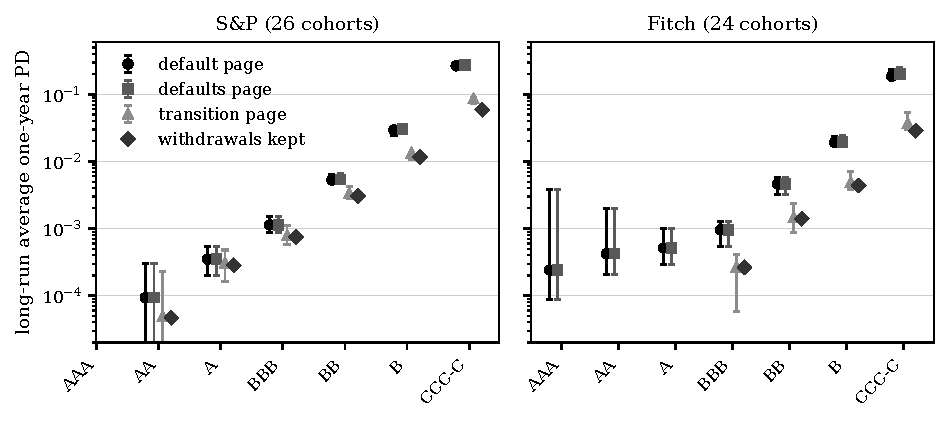
\includegraphics[width=\linewidth]{lra-definitions}
\caption{Long-run average one-year PD by grade of S\&P and Fitch under the default page, the defaults page, the transition page and the transition page with the withdrawals kept, on a logarithmic axis, with the Jeffreys intervals of the pooled counts of the three pages that publish counts; grades with an average of zero are not drawn.}
\label{fig:lra-definitions}
\end{figure}

\begin{figure}[htbp]
\centering
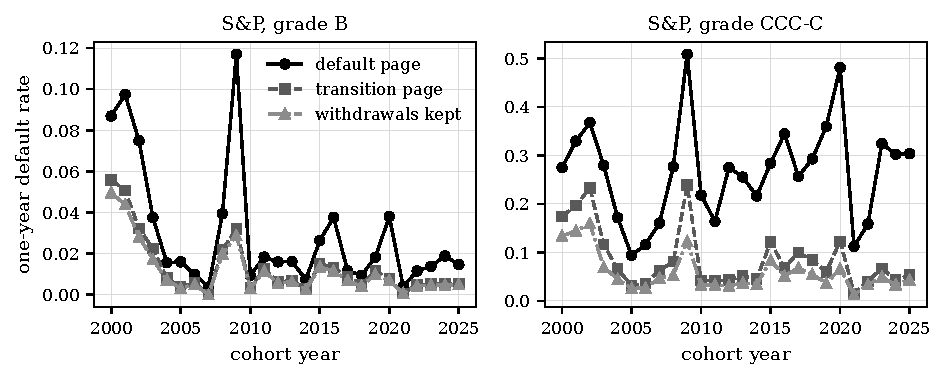
\includegraphics[width=\linewidth]{yearly-gap}
\caption{One-year default rate of S\&P's grades B and CCC to C for each annual cohort from 2000 to 2025 under the default page, the transition page and the transition page with the withdrawals kept, showing that the transition page lies below the default page in every year.}
\label{fig:yearly-gap}
\end{figure}

Figure~\ref{fig:lra-definitions} shows that the gap is largest in the speculative grades, where the withdrawn share and the default rate are both large; in grade A the interval of the gap index of Table~\ref{tab:definitions} includes one, and AA, which has $\spAaNonzeroYears$ year with a nonzero rate, carries no ratio in the table. It does not show why the gap exists. The three explanations that the data cannot separate are the definitions themselves (a rating that defaults and is then withdrawn leaves the transition page's default column), informative withdrawal, and the difference between the cohorts that the pages divide by, which is larger for the default page in $\spGapYears$ of S\&P's years. % voice-ok: withdrawn rating, the domain term of the study

The capital consequence is in Table~\ref{tab:rw} and Figure~\ref{fig:rw-definitions}. The risk weight of S\&P's cohort mix is $\spRwDtwo\%$ with the PDs of the default page and $\spRwDfour\%$ with those of the transition page, a fall of $\spRwGap$ points whose 95\% bootstrap interval is $\spRwGapLo$ to $\spRwGapHi$ and which is positive in $\spRwGapShare\%$ of the $\bootB$ resamples; keeping the withdrawals lowers the weight to $\spRwKeep\%$. For Fitch the weight falls from $\fiRwDtwo\%$ to $\fiRwDfour\%$ ($\fiRwGapLo$ to $\fiRwGapHi$ points), and the transition page's gap index for CCC to C is $\fiPtRatioCcc$ ($\fiRatioCccLo$ to $\fiRatioCccHi$); but these Fitch values carry the defect of the data that Section~\ref{sec:design-data} names: in the $\fiPopDroppedN$ years from \fiPopDropped{} the transition page's default category is empty in every grade, so its rate is zero in those years whatever happened. On the $\fiPopYears$ years in which the category is populated the weight falls from $\fiPopRwDtwo\%$ to $\fiPopRwDfour\%$, a fall of $\fiPopRwGap$ points ($\fiPopRwGapLo$ to $\fiPopRwGapHi$, the last two rows of Table~\ref{tab:rw}), and the gap index for CCC to C is $\fiPopPtRatioCcc$ ($\fiPopRatioCccLo$ to $\fiPopRatioCccHi$), with averages of $\fiPopLraDtwoCcc\%$ and $\fiPopLraDfourCcc\%$. The excess of Fitch's all-years fall over S\&P's is therefore the effect of the empty years, and on the usable years Fitch's gap is of the order of S\&P's. The intervals of the levels overlap in Figure~\ref{fig:rw-definitions}, because the years that raise the rates under one page raise them under the other; the interval of the difference does not, because the resample is common to the definitions. Moody's default page gives $\moLraDtwoCcc\%$ for CCC to C and a weight of $\moRwDtwo\%$, so the default pages of S\&P and Moody's differ by a factor of $\agencyRatio$ for that grade, a spread of the same order as the factor of $\spRatioCccInverse$ that the definitions of S\&P produce. Prediction H1 holds for CCC to C: the upper end of the interval of the gap index is below $0.5$ and the lower end of the risk-weight difference is above zero and above 5 points.

\begin{table}[htbp]
\centering
\setlength{\tabcolsep}{3.5pt}
\footnotesize
\caption{IRB risk weight of each agency's cohort mix (F-IRB corporate, LGD 45\%, maturity 2.5 years, Basel III function) when the one-year PD of every grade is read under each definition, with the percentile interval of 2{,}000 resamples of the cohort years; Moody's transition page has no default category, and the last two rows restrict Fitch to the years in which its transition page's default column is populated.}
\label{tab:rw}
\begin{tabular}{llrrr}
\toprule
Agency & Definition & Risk weight (\%) & 95\% bootstrap interval & Below default page (points) \\
\midrule
\relax S\&P & \relax default page & $58.0$ & \relax [50.0, 65.4] & \relax -- \\
\relax S\&P & \relax defaults page & $58.3$ & \relax [50.3, 65.6] & \relax -- \\
\relax S\&P & \relax transition page & $47.5$ & \relax [40.0, 54.5] & $10.5$ \\
\relax S\&P & \relax withdrawals kept & $45.2$ & \relax [38.2, 52.1] & $12.7$ \\
\relax Moody's & \relax default page & $61.1$ & \relax [49.9, 71.8] & \relax -- \\
\relax Moody's & \relax defaults page & $61.2$ & \relax [50.0, 71.9] & \relax -- \\
\relax Fitch & \relax default page & $46.9$ & \relax [40.7, 56.1] & \relax -- \\
\relax Fitch & \relax defaults page & $47.0$ & \relax [40.9, 56.2] & \relax -- \\
\relax Fitch & \relax transition page & $31.1$ & \relax [26.2, 35.2] & $15.8$ \\
\relax Fitch & \relax withdrawals kept & $30.3$ & \relax [25.5, 34.3] & $16.6$ \\
\relax Fitch & \relax default page, 15 years & $43.8$ & \relax [39.5, 47.7] & \relax -- \\
\relax Fitch & \relax transition page, 15 years & $35.2$ & \relax [30.3, 39.9] & $8.6$ \\
\bottomrule
\end{tabular}
\end{table}


\begin{figure}[htbp]
\centering
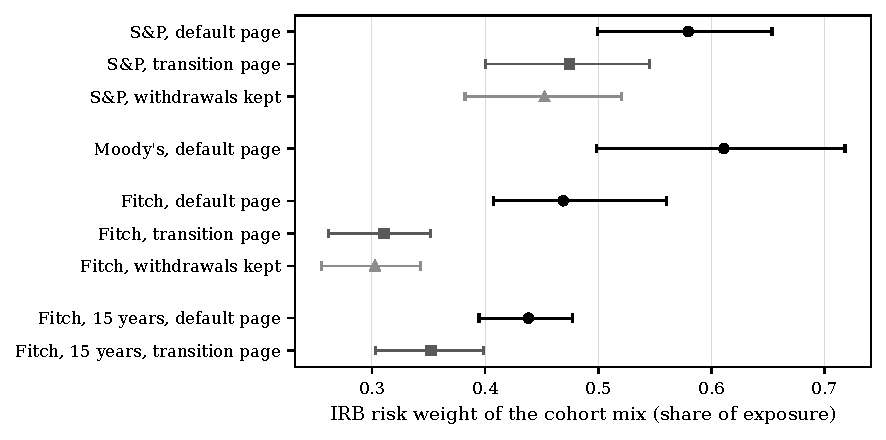
\includegraphics[width=0.92\linewidth]{rw-definitions}
\caption{IRB risk weight of each agency's cohort mix under each definition of the one-year default rate, with the 95\% percentile interval over resamples of the cohort years; Moody's has no transition page default category, so only its default page is shown, and the last two rows restrict Fitch to the years in which its transition page's default category is populated.}
\label{fig:rw-definitions}
\end{figure}

\subsection{Informative withdrawals on paths of known truth}
\label{sec:results-withdrawals}

The committed computation of the case is reproduced to within $\reproMax$ at its four levels of $k$, so the extension rests on the same generator and seeds. Table~\ref{tab:main-results} gives the extension, and Figure~\ref{fig:bias-ladder} plots the bias of grade B against $k$, pooled over five cohorts and on the first cohort alone. At $k=0$, with withdrawal independent of default, removing the withdrawn ratings overstates the PD of B by $\removedBkZero\pm\removedBkZerose$ percent, keeping them understates it by $\keptBkZero\pm\keptBkZerose$ percent, and following them is unbiased ($\followedBkZero\pm\followedBkZerose$), as the first-order formulas predict ($\foRemkZero\%$, $\foKeptkZero\%$ and zero). At $k=1$ the bias of removal has changed sign, $\removedBkOne\pm\removedBkOnese$ percent; at $k=9$, the case the committed computation reports, removal understates the PD by $\removedBkNine\pm\removedBkNinese$ percent, keeping by $\keptBkNine\pm\keptBkNinese$ percent and following by $\followedBkNine\pm\followedBkNinese$ percent (the committed $\repsCommitted$ repetitions gave $\committedremovedkNine\%$, $\committedkeptkNine\%$ and $\committedfollowedkNine\%$). At $k=19$ the removal treatment loses $\removedBkNineteen\pm\removedBkNineteense$ percent of the PD. Grade CCC to C behaves alike: $\removedCcckNine\pm\removedCcckNinese$ percent for removal and $\followedCcckNine\pm\followedCcckNinese$ percent for following at $k=9$. For the lowest grades the estimate is exactly zero in most repetitions (in $\zeroAaaRemoved\%$ of them for AAA with removal at $k=9$), a consequence of the thin cohorts that Section~\ref{sec:results-thin} measures. % voice-ok: withdrawn rating, the domain term of the study

\begin{table}[htbp]
\centering
\setlength{\tabcolsep}{3.5pt}
\footnotesize
\caption{Relative bias (percent of the true one-year PD, mean $\pm$ Monte Carlo standard error over 1{,}000 repetitions) of the pooled cohort estimator with withdrawals removed, kept in the denominator and followed, for grades B and CCC to C, and the error of the IRB risk weight of S\&P's cohort mix (percentage points), against the informativeness $k$ of withdrawal in the year before default.}
\label{tab:main-results}
\resizebox{\linewidth}{!}{\begin{tabular}{rrrrrrrr}
\toprule
$k$ & B removed & B kept & B followed & CCC-C removed & CCC-C followed & Risk weight, removed & Risk weight, followed \\
\midrule
\relax 0 & $2.6\pm0.4$ & $-3.4\pm0.4$ & $-0.2\pm0.4$ & $2.6\pm0.3$ & $-0.3\pm0.3$ & $0.38\pm0.06$ & $-0.09\pm0.06$ \\
\relax 1 & $-2.7\pm0.4$ & $-8.5\pm0.4$ & $-2.3\pm0.4$ & $-1.7\pm0.3$ & $-2.1\pm0.3$ & $-0.42\pm0.06$ & $-0.37\pm0.06$ \\
\relax 2 & $-7.9\pm0.4$ & $-13.4\pm0.3$ & $-4.5\pm0.4$ & $-6.4\pm0.3$ & $-4.5\pm0.3$ & $-1.32\pm0.06$ & $-0.83\pm0.06$ \\
\relax 3 & $-12.0\pm0.4$ & $-17.3\pm0.3$ & $-6.1\pm0.4$ & $-11.2\pm0.3$ & $-7.0\pm0.3$ & $-2.12\pm0.06$ & $-1.15\pm0.06$ \\
\relax 5 & $-20.4\pm0.4$ & $-25.2\pm0.3$ & $-9.2\pm0.4$ & $-19.3\pm0.3$ & $-10.9\pm0.3$ & $-3.55\pm0.06$ & $-1.64\pm0.06$ \\
\relax 9 & $-35.1\pm0.3$ & $-39.2\pm0.3$ & $-15.6\pm0.3$ & $-34.3\pm0.3$ & $-19.0\pm0.3$ & $-6.54\pm0.06$ & $-2.94\pm0.06$ \\
\relax 19 & $-60.3\pm0.3$ & $-62.9\pm0.2$ & $-28.6\pm0.3$ & $-58.9\pm0.2$ & $-33.0\pm0.3$ & $-12.24\pm0.06$ & $-5.35\pm0.06$ \\
\bottomrule
\end{tabular}}
\end{table}


\begin{figure}[htbp]
\centering
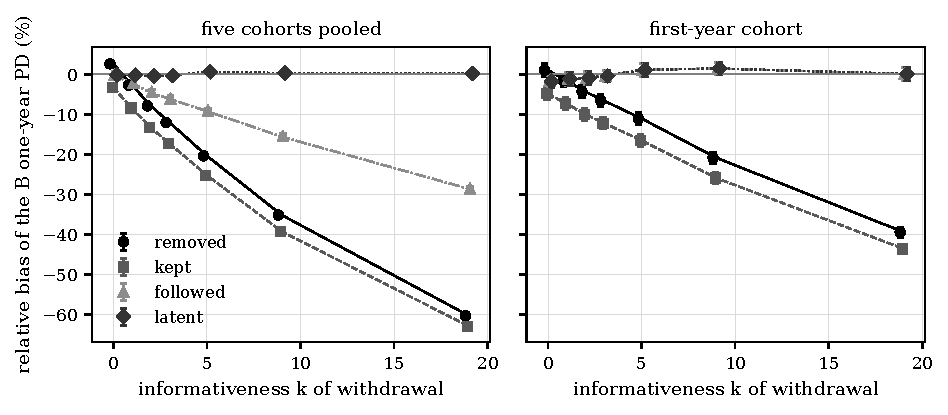
\includegraphics[width=\linewidth]{bias-ladder}
\caption{Relative bias of the one-year PD of grade B against the informativeness of withdrawal for the removal, keeping and following treatments and the no-withdrawal reference, pooled over five annual cohorts (left) and on the first cohort (right), with 95\% intervals from the Monte Carlo standard error of $\repsNew$ repetitions.}
\label{fig:bias-ladder}
\end{figure}

The right panel of Figure~\ref{fig:bias-ladder} is the finding of Proposition~\ref{prop:first-year}. On the first cohort the followed treatment is unbiased at every $k$ (at $k=9$, $\followedYoneBkNine\pm\followedYoneBkNinese$ percent, the sampling noise of the reference), while removal reaches $\removedYoneBkNine\pm\removedYoneBkNinese$ percent and keeping $\keptYoneBkNine\pm\keptYoneBkNinese$ percent. The left panel is the finding of Proposition~\ref{prop:later}: pooling five cohorts adds a bias to the followed treatment that the first cohort did not have. The figure does not show the behaviour of a validator who does not know $k$; the three curves are what each treatment would give at each value of the unknown $k$.

The first-cohort measurements also decide the conjecture of Section~\ref{sec:theory-conjecture}, and they refute it. Table~\ref{tab:conjecture} gives, for the four lowest-rated grades and both treatments, the standardised difference between the measured first-cohort bias and the first-order formula of Equation~\eqref{eq:first-order}. For grade CCC to C the removal treatment differs from the formula by $z=\zCccRemkTwo$, $\zCccRemkFive$ and $\zCccRemkNineteen$ standard errors at $k=2$, $5$ and $19$ (at $k=19$, $\removedYoneCcckNineteen\pm\removedYoneCcckNineteense$ percent against $\foRemkNineteen$ percent); at $k=9$ it is at $z=\zCccRemkNine$, below the criterion of three. For grade B the keeping treatment at $k=19$ differs by $z=\zBKeptkNineteen$ ($\keptYoneBkNineteen\pm\keptYoneBkNineteense$ percent against $\foKeptkNineteen$ percent). Over the grades BBB, BB and B and the levels of $k$ up to nine, the largest difference is $\conjMaxZRestricted$ standard errors over $\conjNRestricted$ comparisons, so that the formula is a usable summary for those grades and levels and not for CCC to C, whose hazard is $\lambdaCcc$ against $\lambdaB$ for B.

\begin{table}[htbp]
\centering
\setlength{\tabcolsep}{3.5pt}
\footnotesize
\caption{Standardised difference $z$ between the measured first-cohort relative bias and the first-order formula of Equation~\eqref{eq:first-order} (measured minus formula, over the Monte Carlo standard error of 1{,}000 repetitions) for the four lowest-rated grades, removal and keeping, at each $k$; a value above three in absolute value, in bold, refutes the conjecture for that case.}
\label{tab:conjecture}
\begin{tabular}{llrrrrrrr}
\toprule
Grade & Treatment & $k=0$ & $k=1$ & $k=2$ & $k=3$ & $k=5$ & $k=9$ & $k=19$ \\
\midrule
\relax BBB & \relax removal & $-0.4$ & $0.1$ & $-0.9$ & $-0.4$ & $-1.2$ & $0.5$ & $-0.0$ \\
\relax BBB & \relax keeping & $-0.4$ & $0.2$ & $-0.9$ & $-0.4$ & $-1.2$ & $0.5$ & $-0.0$ \\
\relax BB & \relax removal & $-0.2$ & $0.0$ & $-0.9$ & $-1.4$ & $-0.7$ & $-1.2$ & $-0.0$ \\
\relax BB & \relax keeping & $-0.2$ & $0.1$ & $-1.0$ & $-1.5$ & $-0.8$ & $-1.3$ & $-0.2$ \\
\relax B & \relax removal & $-2.5$ & $-2.0$ & $-2.0$ & $-1.4$ & $-0.3$ & $-1.0$ & $-1.9$ \\
\relax B & \relax keeping & $-2.5$ & $-2.1$ & $-2.1$ & $-1.6$ & $-0.7$ & $-1.6$ & $\mathbf{-3.1}$ \\
\relax CCC-C & \relax removal & $-1.9$ & $0.1$ & $\mathbf{3.0}$ & $1.2$ & $\mathbf{3.3}$ & $2.8$ & $\mathbf{6.3}$ \\
\relax CCC-C & \relax keeping & $-1.7$ & $-0.1$ & $2.2$ & $0.0$ & $1.2$ & $-0.5$ & $1.0$ \\
\bottomrule
\end{tabular}
\end{table}


The consequence for capital is in the last two columns of Table~\ref{tab:main-results} and in Figure~\ref{fig:rw-error-ladder}. With the true risk weight of the cohort mix at $\rwTruth\%$, the removal treatment lowers it by $\rwAbsremovedkNine$ points at $k=9$ (standard error $\rwremovedkNinese$) and the followed treatment by $\rwAbsfollowedkNine$ points; at $k=19$ the removal error is $\rwremovedkNineteen$ points. The no-withdrawal reference is within $\latentRwMaxZ$ standard errors of zero at every $k$. Prediction H2 holds: at $k=9$ the upper ends of the 95\% intervals of the bias are $\removedBkNine+1.96\times\removedBkNinese$ and $\followedBkNine+1.96\times\followedBkNinese$ percent, both below $-10\%$.

The published estimator that treats a withdrawal as a censoring, the duration estimator, does not escape the bias, as Table~\ref{tab:duration} shows on the same draws. Where withdrawal is independent of default ($k=0$) it is unbiased ($\durBkZero\pm\durBkZerose$ percent for B and $\durCcckZero\pm\durCcckZerose$ for CCC to C, against $\removedBkZero\pm\removedBkZerose$ percent for B with removal), and it estimates a positive PD for AAA ($\zeroAaaDuration\%$ of zero estimates at $k=9$, as at every other level of $k$), where removal returns zero in $\zeroAaaRemoved\%$ of the repetitions at $k=9$. These are the properties for which it is designed. As withdrawal becomes informative it falls below the removal and following treatments, though not below keeping: at $k=9$ it understates the PD of B by $\durBkNine\pm\durBkNinese$ percent and that of CCC to C by $\durCcckNine\pm\durCcckNinese$ percent, against $\removedBkNine\pm\removedBkNinese$ and $\followedBkNine\pm\followedBkNinese$ percent for B under removal and following, and at $k=19$ by $\durBkNineteen\pm\durBkNineteense$ percent; keeping, which divides by the whole cohort, is lower still ($\keptBkNine\pm\keptBkNinese$ percent for B and $\keptCcckNine\pm\keptCcckNinese$ for CCC to C at $k=9$, the kept columns of Table~\ref{tab:duration}). Its bias is thus larger than that of removal and following and smaller than that of keeping. This is the direction expected when withdrawal is more likely before default, a dependence that, as Tsiatis shows, the observed data cannot reveal: the censored paths carry no information on the defaults that the withdrawn ratings would have had, and an estimator that takes the censoring as independent of default cannot recover them. The duration estimator therefore does not repair the bias that the cohort treatments show; the Aalen-Johansen estimator, which makes the same assumption, is not run. % voice-ok: withdrawn rating, the domain term of the study

\begin{table}[htbp]
\centering
\setlength{\tabcolsep}{3.5pt}
\footnotesize
\caption{The duration estimator, which treats a withdrawal as a censoring of the continuous-time path, against the pooled cohort treatments on the same 1{,}000 paired draws: relative bias (percent, mean $\pm$ Monte Carlo standard error) for grades B and CCC to C, and the share of repetitions in which the estimated PD of AAA is exactly zero.}
\label{tab:duration}
\resizebox{\linewidth}{!}{\begin{tabular}{rrrrrrrr}
\toprule
$k$ & B removed & B followed & B duration & CCC-C removed & CCC-C duration & AAA zero, removed (\%) & AAA zero, duration (\%) \\
\midrule
\relax 0 & $2.6\pm0.4$ & $-0.2\pm0.4$ & $-0.4\pm0.3$ & $2.6\pm0.3$ & $-0.3\pm0.3$ & $98.0$ & $0.0$ \\
\relax 1 & $-2.7\pm0.4$ & $-2.3\pm0.4$ & $-5.0\pm0.3$ & $-1.7\pm0.3$ & $-4.9\pm0.3$ & $99.1$ & $0.0$ \\
\relax 2 & $-7.9\pm0.4$ & $-4.5\pm0.4$ & $-10.3\pm0.3$ & $-6.4\pm0.3$ & $-9.6\pm0.3$ & $98.4$ & $0.0$ \\
\relax 3 & $-12.0\pm0.4$ & $-6.1\pm0.4$ & $-14.8\pm0.3$ & $-11.2\pm0.3$ & $-14.0\pm0.3$ & $98.7$ & $0.0$ \\
\relax 5 & $-20.4\pm0.4$ & $-9.2\pm0.4$ & $-22.7\pm0.3$ & $-19.3\pm0.3$ & $-22.1\pm0.3$ & $99.3$ & $0.0$ \\
\relax 9 & $-35.1\pm0.3$ & $-15.6\pm0.3$ & $-37.2\pm0.3$ & $-34.3\pm0.3$ & $-36.8\pm0.2$ & $98.8$ & $0.0$ \\
\relax 19 & $-60.3\pm0.3$ & $-28.6\pm0.3$ & $-61.5\pm0.2$ & $-58.9\pm0.2$ & $-60.8\pm0.2$ & $99.3$ & $0.0$ \\
\bottomrule
\end{tabular}}
\end{table}


\begin{figure}[htbp]
\centering
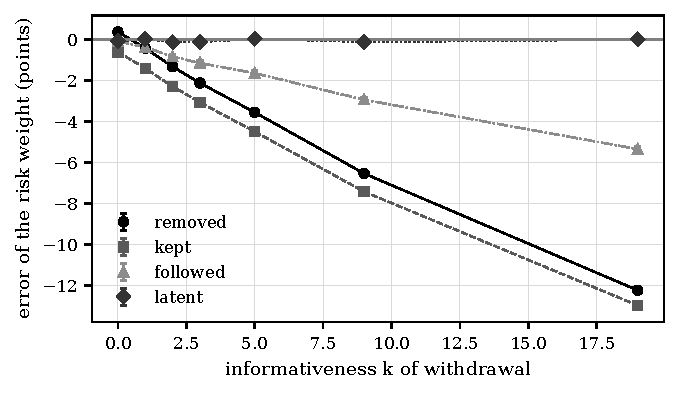
\includegraphics[width=0.72\linewidth]{rw-error-ladder}
\caption{Error, in points, of the IRB risk weight of S\&P's cohort mix computed from the PDs of each treatment of the withdrawn ratings against the informativeness of withdrawal, with 95\% intervals from the Monte Carlo standard error of $\repsNew$ repetitions.} % voice-ok: withdrawn rating, the domain term of the study
\label{fig:rw-error-ladder}
\end{figure}

\subsection{What the transition tests see}
\label{sec:results-tests}

Table~\ref{tab:tests} gives the rejection rates of five transition tests at three levels of $k$ over $\repsTests$ repetitions on the same draws, and Figure~\ref{fig:tests-rejection} plots the first two. At $k=0$ the test of time homogeneity rejects $\testthkZerofive\%$ of the repetitions at the 5\% level (Wilson interval $\testthkZerofivelo$ to $\testthkZerofivehi$) and the test of the last matrix against the true one $\testmrkZerofive\%$ ($\testmrkZerofivelo$ to $\testmrkZerofivehi$), below its level. At $k=9$, where the treatments are $\removedBkNine\%$ and $\followedBkNine\%$ off the truth, the rates are $\testthkNinefive\%$ ($\testthkNinefivelo$ to $\testthkNinefivehi$) and $\testmrkNinefive\%$ ($\testmrkNinefivelo$ to $\testmrkNinefivehi$): the first is within the size of the test plus a fraction, and the second, which compares one year with the truth, is conservative, although its interval at $k=9$ does not overlap its interval at $k=0$, so that it registers a change that it does not turn into a rejection. Neither interval reaches 10\%, so prediction H3 holds as it was stated for these two tests. The three further tests give the following rates at $k=0$, $9$ and $19$: the test of the Markov order $\testordkZerofive\%$, $\testordkNinefive\%$ and $\testordkNineteenfive\%$ (at $k=9$ the Wilson interval is $\testordkNinefivelo$ to $\testordkNinefivehi$, whose upper end is above 10\%), the momentum test $\testmomkZerofive\%$, $\testmomkNinefive\%$ and $\testmomkNineteenfive\%$, and the monotonicity z-tests $\testztkZerofive\%$, $\testztkNinefive\%$ and $\testztkNineteenfive\%$; the Wilson intervals of each of the three overlap across the three levels of $k$. At $k=19$, where removal loses $\removedBkNineteen\%$ of the PD, the time-homogeneity test rejects $\testthkNineteenfive\%$ and the test of the last matrix $\testmrkNineteenfive\%$ ($\testmrkNineteenfivelo$ to $\testmrkNineteenfivehi$), and only then does a test see something. The statement that the prediction rests on, that no matrix test sees the withdrawals, is therefore not held: the test of the last matrix sees them at $k=19$, at a rate whose interval lies well above 10\%. The tests see the withdrawals late, when the bias is already above half the PD, and then at a low rate.

\begin{table}[htbp]
\centering
\setlength{\tabcolsep}{3.5pt}
\footnotesize
\caption{Rejection rates, in percent, of five transition tests of the engine on five annual matrices of the withdrawal generator, over 1{,}000 repetitions per $k$ with Wilson intervals, the same draws for every test at a given $k$; the first two tests are the case's, the other three were run after them, once their results were known. At the level of the test a rate near 5 or 1 means the test does not see the withdrawals; the matrix weighted bandwidth, a descriptive metric with no rejection rule, is not run.}
\label{tab:tests}
\begin{tabular}{lrrr}
\toprule
Transition test & $k$ & Rejections at 5\% (Wilson 95\%) & Rejections at 1\% (Wilson 95\%) \\
\midrule
\relax time homogeneity & \relax 0 & $2.8$ [1.9, 4.0] & $0.4$ [0.2, 1.0] \\
\relax time homogeneity & \relax 9 & $5.8$ [4.5, 7.4] & $1.0$ [0.5, 1.8] \\
\relax time homogeneity & \relax 19 & $8.8$ [7.2, 10.7] & $2.1$ [1.4, 3.2] \\
\relax last year against $\exp(Q)$ & \relax 0 & $0.2$ [0.1, 0.7] & $0.0$ [0.0, 0.4] \\
\relax last year against $\exp(Q)$ & \relax 9 & $1.4$ [0.8, 2.3] & $0.0$ [0.0, 0.4] \\
\relax last year against $\exp(Q)$ & \relax 19 & $16.3$ [14.1, 18.7] & $4.3$ [3.2, 5.7] \\
\relax Markov order & \relax 0 & $6.0$ [4.7, 7.6] & $2.2$ [1.5, 3.3] \\
\relax Markov order & \relax 9 & $8.3$ [6.7, 10.2] & $2.5$ [1.7, 3.7] \\
\relax Markov order & \relax 19 & $6.6$ [5.2, 8.3] & $3.2$ [2.3, 4.5] \\
\relax rating momentum & \relax 0 & $4.2$ [3.1, 5.6] & $0.7$ [0.3, 1.4] \\
\relax rating momentum & \relax 9 & $4.2$ [3.1, 5.6] & $0.8$ [0.4, 1.6] \\
\relax rating momentum & \relax 19 & $4.1$ [3.0, 5.5] & $0.5$ [0.2, 1.2] \\
\relax monotonicity z-tests & \relax 0 & $0.0$ [0.0, 0.4] & $0.0$ [0.0, 0.4] \\
\relax monotonicity z-tests & \relax 9 & $0.0$ [0.0, 0.4] & $0.0$ [0.0, 0.4] \\
\relax monotonicity z-tests & \relax 19 & $0.1$ [0.0, 0.6] & $0.0$ [0.0, 0.4] \\
\bottomrule
\end{tabular}
\end{table}


\begin{figure}[htbp]
\centering
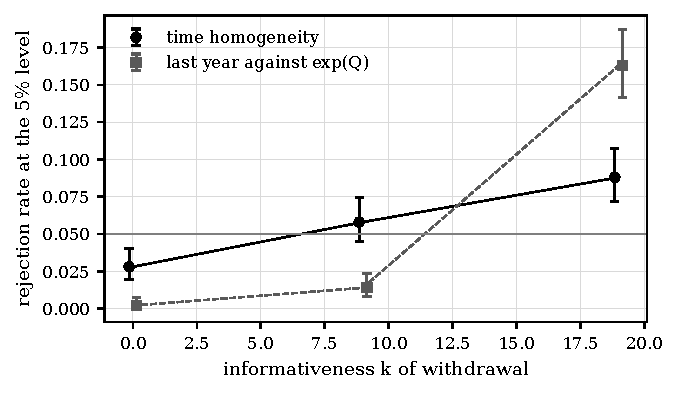
\includegraphics[width=0.72\linewidth]{tests-rejection}
\caption{Rejection rate at the 5\% level of the test of time homogeneity across five annual matrices and of the test of the last matrix against the true one-year matrix, against the informativeness of withdrawal, with Wilson intervals over $\repsTests$ repetitions; the horizontal line is the level of the test.}
\label{fig:tests-rejection}
\end{figure}

\subsection{Thin grades by exact enumeration}
\label{sec:results-thin}

Table~\ref{tab:thin} and Figure~\ref{fig:thin-coverage} give the exact coverage. With 50 obligors per grade the Wald interval contains the PD of AAA in $\waldAaaFifty\%$ of the samples ($\waldAaaFiftyFour\%$ to four digits), of AA in $\waldAaFifty\%$, and in $\waldBbbFifty\%$ of BBB, $\waldBFifty\%$ of B and $\waldCccFifty\%$ of CCC to C. The Agresti-Coull and Jeffreys intervals cover at least $\acMinFifty\%$ and $\jeffMinFifty\%$ in every grade at that size, so the statement of H4 is reproduced in both clauses (the case's committed enumeration is the source of these values, and nothing in this paper's own computation could have refuted them). The price is the width: at the PD of AAA the expected lengths at 50 obligors are $\lenWaldAaaFifty$ basis points for the Wald interval, $\lenJeffAaaFifty$ for the Jeffreys interval and $\lenAcAaaFifty$ for the Agresti-Coull interval, against a PD of $\pAaaBp$ basis points. At 1,000 obligors the Wald interval covers the PD of AAA in $\waldAaaThou\%$ of the samples, and the Jeffreys interval covers $\jeffThouAaa\%$ for AAA, $\jeffThouBb\%$ for BB, $\jeffThouB\%$ for B and $\jeffThouCcc\%$ for CCC to C, below the nominal level, and $\jeffThouAa\%$, $\jeffThouA\%$ and $\jeffThouBbb\%$ for AA, A and BBB, at or above it, as Table~\ref{tab:thin} shows. The shortfall therefore does not follow the thinness of the grade: it falls on AAA and on three of the thicker grades and spares AA, the grade with the lowest PD, because the coverage of the Jeffreys interval oscillates with the number of obligors, the behaviour that Brown, Cai and DasGupta describe for the interval \citep{Brown_2001}. At the cohort sizes of the generator the Wald coverage is $\waldAaaGen\%$ for AAA, $\waldAaGen\%$ for AA and $\waldAGen\%$ for A. The grid of Figure~\ref{fig:thin-coverage} locates the size at which the Wald interval reaches 90\%: $\waldFirstBb$ obligors for BB, $\waldFirstCcc$ for CCC to C, and for AAA no size of the grid up to $\gridMax$ obligors (at $\gridMax$ the coverage is $\waldAaaFiftyK\%$). The grades cannot be told apart in the investment range: at 1,000 obligors the Jeffreys intervals of AAA and AA overlap with probability $\overlapAaaAaThou$, while B and CCC to C separate from 200 obligors (overlap $\overlapBCccTwo$).

\begin{table}[htbp]
\centering
\setlength{\tabcolsep}{3.5pt}
\footnotesize
\caption{Exact coverage (percent, nominal 95) of the Wald, Agresti-Coull and Jeffreys intervals at the true one-year PD of each grade, by enumeration of the binomial count, with 50 and 1{,}000 obligors per grade and at the cohort sizes of the S\&P-like generator; the PDs are those of the C04 generator.}
\label{tab:thin}
\resizebox{\linewidth}{!}{\begin{tabular}{lrrrrrrrrrr}
\toprule
Grade & $p$ (\%) & Wald, 50 & A-C, 50 & Jeffreys, 50 & Wald, 1000 & A-C, 1000 & Jeffreys, 1000 & Cohort size & Wald, size & Jeffreys, size \\
\midrule
\relax AAA & $0.007$ & $0.3$ & $100.0$ & $99.7$ & $6.4$ & $100.0$ & $93.6$ & \relax 75 & $0.5$ & $99.5$ \\
\relax AA & $0.005$ & $0.2$ & $100.0$ & $99.8$ & $4.8$ & $100.0$ & $95.2$ & \relax 822 & $4.0$ & $96.0$ \\
\relax A & $0.029$ & $1.4$ & $100.0$ & $98.6$ & $25.1$ & $99.7$ & $96.6$ & \relax 1814 & $40.7$ & $98.4$ \\
\relax BBB & $0.082$ & $4.0$ & $99.9$ & $96.0$ & $55.8$ & $99.0$ & $95.0$ & \relax 1756 & $76.1$ & $98.4$ \\
\relax BB & $0.346$ & $15.9$ & $99.9$ & $98.7$ & $85.7$ & $97.5$ & $94.4$ & \relax 1054 & $87.5$ & $94.1$ \\
\relax B & $1.173$ & $44.5$ & $97.9$ & $97.9$ & $93.9$ & $96.1$ & $94.6$ & \relax 1391 & $92.5$ & $95.6$ \\
\relax CCC-C & $8.062$ & $91.4$ & $95.5$ & $96.8$ & $94.7$ & $95.2$ & $94.5$ & \relax 201 & $92.6$ & $94.6$ \\
\bottomrule
\end{tabular}}
\end{table}


\begin{figure}[htbp]
\centering
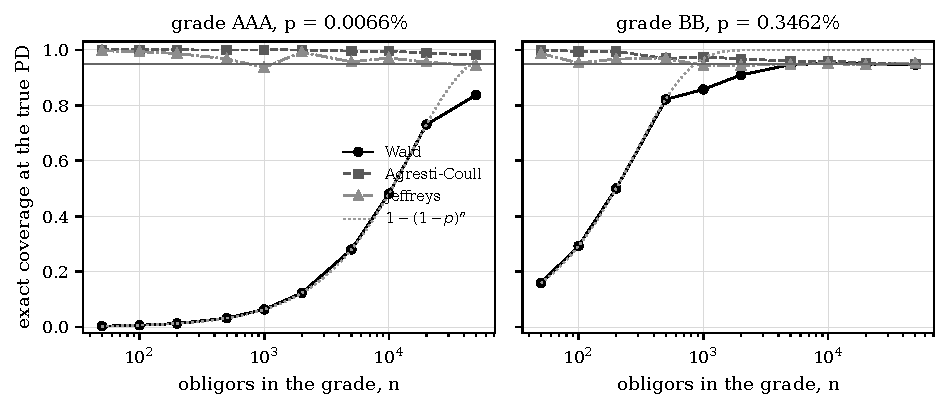
\includegraphics[width=\linewidth]{thin-coverage}
\caption{Exact coverage at the true PD of the Wald, Agresti-Coull and Jeffreys intervals against the number of obligors in the grade, for AAA (left) and BB (right), with the closed form $1-(1-p)^n$ of the Wald coverage as a dotted line and the nominal 95\% as a horizontal line.}
\label{fig:thin-coverage}
\end{figure}

\subsection{The closed forms and the numerical evaluations against the simulation}
\label{sec:results-theory}

Table~\ref{tab:theory} and Figure~\ref{fig:theory-vs-simulation} compare the closed forms of Section~\ref{sec:theory} with the engine's simulation on the two-state chain with the PD of grade B. The largest standardised difference is $\thMaxZFirst$ over the $\thNcmpFirst$ distinct first-cohort comparisons, which test the closed forms of Proposition~\ref{prop:first-year} (H5a), and $\thMaxZPooled$ over the $\thNcmpPooled$ pooled comparisons, which test the numerical evaluation of the model's masses and not a closed form (H5b); the two chains, five levels of $k$, four estimators including the reference and two scopes make $\thNcmp$ entries, of which $\thNcmpDistinct$ are distinct because the first-cohort followed estimator and the reference read the same draws and have the same value. Predictions H5a and H5b hold. The two-state chain does not carry over to the multi-state grades in one direction, and the direction differs between grades. For grade B, the two-state numerical evaluation for the removal treatment pooled over five cohorts at $k=9$ is $\thBremovedPoolkNine\%$, against $\removedBkNine\pm\removedBkNinese\%$ on the multi-state generator of S\&P-like cohorts ($\zTwoStateremovedB$ standard errors apart), whereas for following it gives $\thBfollowedPoolkNine\%$ against $\followedBkNine\pm\followedBkNinese\%$ ($\zTwoStatefollowedB$ standard errors), so that the two-state evaluation overstates the selection bias of the followed treatment. For grade CCC to C it goes the other way for both treatments: removal $\thCccremovedPoolkNine\%$ against $\removedCcckNine\pm\removedCcckNinese\%$ ($\zTwoStateremovedCcc$ standard errors) and following $\thCccfollowedPoolkNine\%$ against $\followedCcckNine\pm\followedCcckNinese\%$ ($\zTwoStatefollowedCcc$ standard errors), that is, the two-state evaluation understates the bias. The sign of the two-state error therefore differs between grade B and grade CCC to C, and the two-state model is a guide to the mechanism and not a substitute for the measurement on the grade at hand. The figure shows the agreement between the closed forms and the two-state simulation for the three treatments in both scopes.

\begin{table}[htbp]
\centering
\setlength{\tabcolsep}{3.5pt}
\footnotesize
\caption{The closed forms of the Theory section (first cohort) and the numerical evaluation of the model's masses (pooled over five cohorts) against the engine's simulation on a two-state chain with the PD of grade B (relative bias of the one-year PD in percent; the simulated value is the mean $\pm$ Monte Carlo standard error of 40 paired draws of 100{,}000 obligors, $z$ the standardised difference).}
\label{tab:theory}
\resizebox{\linewidth}{!}{\begin{tabular}{rlrrrrrr}
\toprule
$k$ & Estimator & Pooled: numerical evaluation & Pooled: simulated & $z$ & First year: closed form & First year: simulated & $z$ \\
\midrule
\relax 0 & \relax removed & $3.0$ & $3.0\pm0.2$ & $0.02$ & $3.0$ & $2.9\pm0.5$ & $-0.28$ \\
\relax 0 & \relax kept & $-2.9$ & $-2.9\pm0.2$ & $0.04$ & $-2.9$ & $-3.1\pm0.4$ & $-0.26$ \\
\relax 0 & \relax followed & $0.0$ & $0.0\pm0.2$ & $0.08$ & $0.0$ & $-0.2\pm0.5$ & $-0.35$ \\
\relax 1 & \relax removed & $-2.2$ & $-2.0\pm0.2$ & $1.06$ & $0.1$ & $-0.2\pm0.4$ & $-0.72$ \\
\relax 1 & \relax kept & $-7.9$ & $-7.7\pm0.2$ & $1.13$ & $-5.8$ & $-6.0\pm0.4$ & $-0.64$ \\
\relax 1 & \relax followed & $-2.2$ & $-2.1\pm0.2$ & $0.83$ & $0.0$ & $-0.3\pm0.4$ & $-0.87$ \\
\relax 3 & \relax removed & $-11.8$ & $-11.7\pm0.2$ & $0.46$ & $-5.4$ & $-5.3\pm0.5$ & $0.16$ \\
\relax 3 & \relax kept & $-17.1$ & $-17.0\pm0.2$ & $0.43$ & $-11.1$ & $-11.0\pm0.5$ & $0.13$ \\
\relax 3 & \relax followed & $-6.5$ & $-6.5\pm0.1$ & $0.05$ & $0.0$ & $0.1\pm0.5$ & $0.18$ \\
\relax 9 & \relax removed & $-35.0$ & $-35.2\pm0.2$ & $-1.18$ & $-19.7$ & $-19.7\pm0.4$ & $0.05$ \\
\relax 9 & \relax kept & $-39.0$ & $-39.2\pm0.2$ & $-1.16$ & $-24.8$ & $-24.7\pm0.4$ & $0.06$ \\
\relax 9 & \relax followed & $-17.4$ & $-17.7\pm0.2$ & $-1.59$ & $0.0$ & $-0.1\pm0.5$ & $-0.18$ \\
\relax 19 & \relax removed & $-60.0$ & $-59.9\pm0.1$ & $0.39$ & $-37.5$ & $-37.4\pm0.4$ & $0.28$ \\
\relax 19 & \relax kept & $-62.6$ & $-62.5\pm0.1$ & $0.39$ & $-41.7$ & $-41.6\pm0.4$ & $0.25$ \\
\relax 19 & \relax followed & $-30.9$ & $-30.8\pm0.2$ & $0.15$ & $0.0$ & $0.8\pm0.5$ & $1.69$ \\
\bottomrule
\end{tabular}}
\end{table}


\begin{figure}[htbp]
\centering
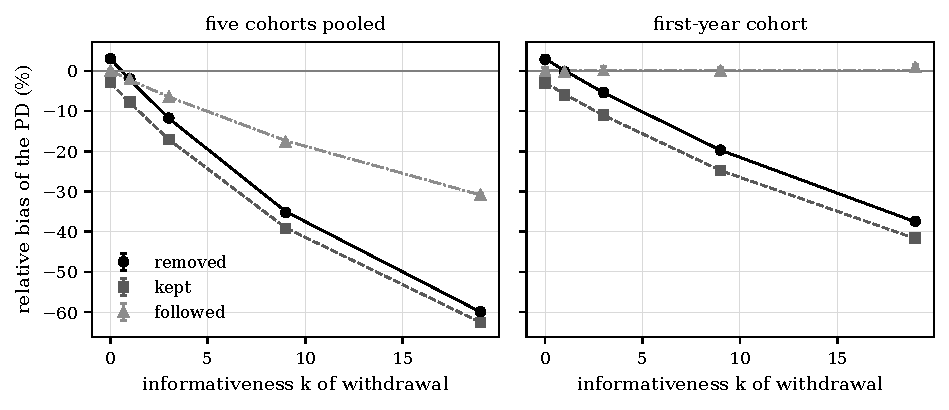
\includegraphics[width=\linewidth]{theory-vs-simulation}
\caption{Relative bias of the one-year PD of a two-state chain with the PD of grade B against the informativeness of withdrawal: the numerical evaluations (pooled, left) and the closed forms (first cohort, right) of the Theory section as lines and the means of the engine's simulation as points with 95\% intervals, pooled over five cohorts (left) and on the first cohort (right).}
\label{fig:theory-vs-simulation}
\end{figure}

\subsection{Outcome of the predictions}
\label{sec:results-outcomes}

Table~\ref{tab:outcomes} lists the predictions and the conjecture with their deciding quantity and their outcome. H1, H2 and the two parts of H5 hold; H4 is reproduced and could not have failed; H3 holds for the two tests at $k=9$ for which it was stated, but the statement behind it does not, because the test of the last matrix rejects in $\testmrkNineteenfive\%$ of the repetitions at $k=19$; and the conjecture is refuted for CCC to C and, at $k=19$, for keeping in grade B. Four details temper the reading. The gap index of grade B at S\&P is not below one half with confidence, so the claim of H1 is made for CCC to C only. The first-order formula of Equation~\eqref{eq:first-order} is refuted for grade CCC to C at three of the seven levels of $k$ (and at $k=9$ it is just under the criterion), and the exact closed form is needed there. The two-state numerical evaluation misses the multi-state followed treatment in both grades, in opposite directions. And the Jeffreys interval, which satisfies the statement of H4 at 50 obligors, is below its nominal coverage at 1,000 obligors in the grades AAA, BB, B and CCC to C, and above it in AA, A and BBB. The outcomes therefore support the statement that the three conventions move the PD, but they support the sharper claims only within the conditions listed: a speculative grade for the gap, a level of informativeness at or above one for the sign of the bias, a PD of about $1.2\%$ or less and a level of informativeness up to nine for the first-order formula, and a cohort whose expected default count is below one for the shortfall of the Wald coverage.

\begin{table}[htbp]
\centering
\setlength{\tabcolsep}{3.5pt}
\footnotesize
\caption{The predictions of the experimental design and the outcome of each: the four statements of the measurements on the default definition, informative withdrawals and thin grades, the closed forms of the Theory section, and the conjecture of that section, with the quantity that decides each.}
\label{tab:outcomes}
\begin{tabular}{lp{5.2cm}p{4.2cm}p{2.6cm}}
\toprule
Id & Prediction & Result & Outcome \\
\midrule
\relax H1 & \relax On S\&P's CEREP cohorts the transition page's long-run PD of CCC to C is below one half of the default page's (95\% interval of the ratio below 0.5), and the risk weight of the cohort mix falls by more than 5 points & $0.323$ [0.259, 0.391]; $10.5$ points [8.3, 13.1] & \relax held (the point values reproduce the committed ones; the bootstrap interval is new) \\
\relax H2 & \relax With $k=9$ the pooled B PD with withdrawals removed and with withdrawals followed are each at least 10\% below the truth (95\% interval of the relative bias below $-10$\%) & \relax removed $-35.1\pm0.3$, followed $-15.6\pm0.3$ & \relax held \\
\relax H3 & \relax At $k=9$ neither the test of time homogeneity nor the test of the last matrix rejects more than 10\% of the repetitions at the 5\% level (upper Wilson bound below 10\%). The statement behind it, that no transition test of the engine sees the withdrawals, is refuted by a rate whose lower bound is above 10\% at any $k$ or any test & $k=9$: $5.8$ [4.5, 7.4] and $1.4$ [0.8, 2.3]; last matrix at $k=19$: $16.3$ [14.1, 18.7]; Markov order at $k=9$: $8.3$ [6.7, 10.2] & \relax held for the two tests at $k=9$; the statement is not held, the last-matrix test sees the withdrawals at $k=19$ \\
\relax H4 & \relax With 50 obligors the Wald interval covers the PD of AAA in $0.33\%$ of the samples (to two digits) and the Jeffreys and Agresti-Coull intervals cover at least 95\% in every grade & \relax Wald $0.33$\%; minimum $96.0$\% (Jeffreys), $95.5$\% (A-C) & \relax reproduced (an exact enumeration of values already committed; it could not fail) \\
\relax H5a & \relax The closed forms of Proposition~\ref{prop:first-year} agree with the simulated means of the first cohort within three Monte Carlo standard errors & \relax largest $|z|=1.69$ over 30 distinct comparisons & \relax held \\
\relax H5b & \relax The numerical evaluation of the model's masses over five cohorts, with the horizon truncation, agrees with the pooled simulated means within three Monte Carlo standard errors & \relax largest $|z|=1.59$ over 40 distinct comparisons & \relax held \\
\relax Conj. & \relax The first-order formula of Equation~\eqref{eq:first-order} describes the first-cohort bias of a grade with a small PD to within three standard errors & \relax CCC to C, removal: $z=3.02$, $3.31$, $6.32$ at $k=2,5,19$; B, keeping, $k=19$: $z=-3.07$ & \relax refuted for CCC to C and, at $k=19$, for keeping in B \\
\bottomrule
\end{tabular}
\end{table}



\section{Ablation}
\label{sec:ablation}
Table~\ref{tab:ablation} removes one component of the protocol at a time and reports, on the same data, the quantity that the component makes visible, with the component and without it. The ablation is one at a time: it does not measure interactions between components.

\begin{table}[htbp]
\centering
\setlength{\tabcolsep}{3.5pt}
\footnotesize
\caption{Ablation of the proposed protocol: each row removes one component and reports, on the same data, the quantity the component makes visible; the first two rows read the committed CEREP artifacts, the next four the known-truth draws, the last two the exact enumeration and the matrix tests.}
\label{tab:ablation}
\resizebox{\linewidth}{!}{\begin{tabular}{p{3.2cm}p{2.6cm}p{3.2cm}p{2.4cm}p{3cm}}
\toprule
Component of the protocol & Without it & Quantity & With the component & Without the component \\
\midrule
\relax Report the three pages' definitions side by side & \relax Report the transition page only & \relax S\&P CCC to C, long-run PD (\%) & $26.64$ and $8.61$ & $8.61$ (the gap is not seen) \\
\relax The same, carried to capital & \relax Report the transition page only & \relax S\&P risk weight (\%) & $58.0$ and $47.5$ & $47.5$ ($10.5$ points lower) \\
\relax Informativeness ladder of $k$ & \relax Run $k=0$ only & \relax B, removed estimator, relative bias (\%) & $-35.1\pm0.3$ at $k=9$ & $2.6\pm0.4$ at $k=0$ (opposite sign) \\
\relax Known-truth reference & \relax Compare the three treatments with one another & \relax B at $k=9$: bias of the least biased treatment (followed) & $-15.6\pm0.3$ against the truth & \relax treatments span $23.7$ points; the offset of every one from the truth is unknown \\
\relax First-year cohort alone & \relax Pool five annual cohorts & \relax B, followed estimator, relative bias at $k=9$ (\%) & $1.4\pm0.8$ (first year) & $-15.6\pm0.3$ (pooled) \\
\relax Paired observed and latent draws & \relax Independent draws & \relax Standard error of removed minus latent, B, $k=9$ ($10^{-5}$) & $3.0$ & $5.6$ \\
\relax Exact enumeration of the coverage & \relax Estimate the coverage by simulation & \relax Repetitions to resolve the Wald coverage of AAA at $n=50$ to 10\% relative error & \relax 0 (exact) & $30{,}400$ \\
\relax Matrix tests as the screen for withdrawals & \relax None needed (no screen) & \relax Rejection rate at 5\% of the weaker test at $k=9$ (\%) & $1.4$ and $5.8$ & \relax the screen rejects at about its size, and the bias is not seen \\
\bottomrule
\end{tabular}}
\end{table}


The first two rows concern the definition-explicit report. A validator who reads only the transition page sees $\spLraDfourCcc\%$ for CCC to C where the default page shows $\spLraDtwoCcc\%$, and a risk weight of $\spRwDfour\%$ where the default page gives $\spRwDtwo\%$, $\spRwGap$ points lower. Nothing in the transition page reveals the difference, because the counts that would reveal it are on another page. The component costs nothing to run, since the pages are published together, and it supplies the largest single effect of the protocol on capital.

The third row concerns the ladder of informativeness. At $k=0$ the removal treatment overstates the PD of B by $\removedBkZero\pm\removedBkZerose$ percent, a result from which a validator would conclude that the industry convention is slightly conservative; at $k=9$ the same estimator understates the PD by $\removedBkNine\pm\removedBkNinese$ percent. The sign changes between $k=0$ and $k=1$. A measurement at one level of $k$ gives an answer that depends on the level chosen, and the ladder shows that dependence.

The fourth row concerns the reference to the known truth. Without the truth, the three treatments can only be compared with one another; at $k=9$ they span $\keptBkNine\%$ to $\followedBkNine\%$ and the one with the smallest bias, the followed treatment, would be taken as the reference, although it is itself below the truth by $\followedBkNine\pm\followedBkNinese$ percent. The error of the best treatment is invisible without the truth.

The fifth row concerns pooling. The followed treatment is exact on the first cohort ($\followedYoneBkNine\pm\followedYoneBkNinese$ percent at $k=9$) and biased by $\followedBkNine\pm\followedBkNinese$ percent when five cohorts are pooled, which is the selection of Proposition~\ref{prop:later}. Pooling is the practice that the long-run average of paragraph 84 of the guidelines invites, and the ablation shows the cost for the treatment that otherwise has none.

The sixth row concerns the pairing of the observed and latent draws. The standard error of the contrast between the removal estimator and the reference at $k=9$ for grade B is $\seRemovedPaired\times10^{-5}$ with pairing and $\seRemovedUnpaired\times10^{-5}$ without, a ratio of $\seRatio$, so pairing removes $\seRatioPct\%$ of the standard error of the contrast, or equivalently the pairing is worth about $\seRatio^2$ times as many repetitions. The seventh row concerns the enumeration. To resolve a Wald coverage of $\waldAaaFifty\%$ to a relative error of 10\% by simulation takes about $\repsNeeded$ repetitions, whereas the enumeration is exact; the more important gain is that a simulation of $\repsNew$ repetitions cannot distinguish a coverage of $\waldAaaFifty\%$ from zero. The eighth row concerns the screen: the matrix tests reject $\testthkNinefive\%$ and $\testmrkNinefive\%$ of the repetitions at $k=9$, no more than their size, so they would add nothing to a decision about withdrawals there, and the known-truth measurement is what reveals the bias.


\section{Discussion}
\label{sec:discussion}
\subsection{Why the results are what they are}
\label{sec:discussion-why}

The results have three separate origins, and the protocol measures each separately. The gap between the pages is a matter of counting. The default page counts a rating that defaulted whatever its position at the end of the year; the transition page counts only the ratings that are in a default category at the end, and a rating that defaults and is then withdrawn is in the withdrawals column. The speculative grades, where defaulted ratings are withdrawn at the end of the window in the case's lifetime check, therefore lose defaults from the transition page, and the loss is large exactly where the default rate is large. The data cannot separate this from informative withdrawal, because both remove would-be defaults from the numerator, and the real cohorts alone cannot say how much of the $\spLraDtwoCcc\%$ to $\spLraDfourCcc\%$ difference is which.

The bias of the treatments is a matter of selection. Proposition~\ref{prop:first-year} shows that a rating about to default is exposed, during the part of its last year that lies inside the cohort year, to a hazard of withdrawal $1+k$ times the baseline, so withdrawal is a competing event that hides defaults; Proposition~\ref{prop:later} shows that the same hazard acts a year ahead, so that the cohort of the next year is already short of the ratings about to default. The first effect is why removal and keeping are biased on the first cohort, and the second why the followed treatment is biased after it. Both are visible in the closed forms, and both are measured: the two-state closed form for the removal treatment at $k=9$ is within one standard error of the multi-state measurement.

The thin-grade results are a matter of discreteness. When the expected number of defaults in a grade is below one, the observed rate is zero in most samples, and an interval built on the observed rate cannot contain a positive PD (Proposition~\ref{prop:wald}); an interval that is centred elsewhere, as the Jeffreys and Agresti-Coull intervals are, contains the PD in the samples with no default and so reaches nominal coverage at the cost of a width of several hundred basis points around a PD of less than one.

\subsection{What a validator can do with them}
\label{sec:discussion-use}

Four practices follow from the measurements, each within what the data can support. A PD from agency statistics should carry the name of the page it was read from; the gap index of Equation~\eqref{eq:gap-index} and the risk-weight difference show what the alternative would have been. A treatment of withdrawn ratings should be chosen with the first cohort in view: where the end of every rating can be followed, as in the bank's own data, the followed treatment applied to a single cohort is unbiased in the model, and pooling cohorts reintroduces a selection bias that is a function of the informativeness. For a grade with an expected default count below about three, the Wald interval should not be reported; the Jeffreys interval covers, and its width states how little is known. And the matrix tests should not be taken as evidence against informative withdrawal: at levels of informativeness at which the PD is already wrong by a third they reject at rates of the order of their size.

The measurement does not say which page is right, or which value of $k$ holds for a given agency. It gives the range within which the PD moves, and the value of the range for capital is what a validator needs to size a margin of conservatism: at $k=9$ the removal treatment lowers the risk weight of S\&P's cohort mix by $\rwAbsremovedkNine$ points, which sets the order of magnitude for an adjustment of the risk weight if the withdrawals of the portfolio are suspected to be informative. A method that repairs the bias needs more than the transition page: it must anchor the informativeness on a second count of defaults, or report the PD as a function of $k$ with the value at which a decision flips. The engine of the case provides that family of estimates, and its evaluation is a separate study; the present measurement is what such an estimator has to beat.

\subsection{Negative and partial results}
\label{sec:discussion-negative}

Six results go against the simple story. The first is that the gap index of grade B at S\&P cannot be said to be below one half, so the strongest form of the claim holds for CCC to C only. The second is that following the withdrawn ratings, the treatment the guidelines ask for, is biased by $\followedBkNine\pm\followedBkNinese$ percent at $k=9$ once cohorts are pooled; its exactness on the first cohort does not carry over. The third is that the matrix tests do not see the withdrawals at $k=9$ and see them at only $\testmrkNineteenfive\%$ at $k=19$ with the better of the two. The fourth is that the first-order formula of the Theory section overstates the bias of grade CCC to C, where the PD is too large for a first-order expansion. The fifth is that the two-state closed form overstates the selection bias of the followed treatment on the multi-state generator ($\thBfollowedPoolkNine\%$ against $\followedBkNine\pm\followedBkNinese\%$), so the closed forms are a guide to the mechanism and not a substitute for the measurement on the grade at hand. The sixth is that the Jeffreys interval, the interval that behaves best at 50 obligors, is below nominal coverage in the thinnest grades at 1{,}000 obligors, because the enumeration of its coverage at a rare PD oscillates with $n$ and is not monotone.


\section{Limitations}
\label{sec:limitations}
\subsection{Internal validity}
\label{sec:limitations-internal}

The thresholds of the predictions were set with the committed values in view: the ratio of one half for the gap index, the bias of $-10\%$ for the treatments, the rejection rate of 10\% for the tests. The new seeds of the extension guard against a dependence on the seed of the committed computation; they do not guard against the choice of thresholds. The interval of the gap index and of the risk-weight difference resamples the annual cohorts as if they were independent, whereas rating statistics have serial dependence through the cycle; a block resample would widen the interval \citep{Kunsch_1989}, and the intervals reported are therefore likely too narrow for the real-data comparison. The Monte Carlo standard errors of the known-truth results are small ($\removedBkNinese$ percent for the bias of B at $k=9$) and cover the sampling of the generator only, not the estimation error of the generator, which is itself fitted to S\&P's counts. The transition tests were run at three levels of $k$ only, and three of the five were run after the first two, once their results were known; the threshold of 10\% for H3 was fixed with the committed rates in view, and the statement that no matrix test sees the withdrawals was tested more narrowly than it was made until the further tests were run. The duration estimator is measured on one generator and one withdrawal window, and the Aalen-Johansen estimator is not measured. The restricted form of the conjecture of Section~\ref{sec:theory-conjecture} is a description of the same measurements, not a test.

\subsection{External validity}
\label{sec:limitations-external}

The known-truth results hold for the generator they were run on: a Markov chain fitted to S\&P's pooled annual counts, cohorts of the size of S\&P's mean cohort, a baseline withdrawal rate of $\wRate\%$ a year and an elevated window of one year before default. A different agency, a different rate or window, or an informative mechanism that acts through the rating path rather than through the time to default would give different biases; the closed forms give the direction and the order of magnitude, and the measurement has to be repeated for each. The real-data results hold for the corporate long-term ratings of the EU entities of three agencies, in the categories scale, for 2000 to 2025; they do not extend to the agencies' global books, to other asset classes or to the notch scale. No data say whether withdrawals of real ratings were informative, and the value $k=9$ is a point on the ladder, not an estimate.

\subsection{Construct validity}
\label{sec:limitations-construct}

Four constructs deserve care. First, the followed treatment is the product's reading of paragraphs 73 and 76 of the guidelines at the one-year level, in which the end state of every rating outstanding at the start is read on the latent path; the guidelines speak of obligors and credit obligations, and the repository counts ratings. Second, the gap between the pages mixes the definition, informative withdrawal and the difference between the cohorts, and the protocol cannot separate them on real data. Third, the risk weight is that of a foundation-approach corporate exposure with a loss given default of $45\%$, a maturity of $2.5$ years, the Basel III function and the PD floor, applied to a portfolio whose grade mix is that of the agency's mean cohort; a bank's portfolio and parameters differ, so the risk-weight differences are an illustration of the size of the effect and not a capital figure. Fourth, the long-run average is the mean of annual rates, as paragraph 84 states, which weights each year equally whatever its cohort; the pooled rates of the same counts differ from it in the speculative grades.

\subsection{Scope}
\label{sec:limitations-scope}

The protocol is a measurement and does not repair the bias it finds. It uses synthetic obligors for the truth and so does not test the treatments on a bank's own data, where the follow-up of withdrawn obligations may be available. It reports the PD of a grade over one year and does not carry the conclusions to multi-year horizons, where the chain of one-year matrices compounds the bias. The thin-grade results assume that the cohort is a set of independent obligors with one PD, which the binomial enumeration requires; with default correlation the coverage would be lower still, and the dependence correction of the effective cohort size, which the engine provides for the Wald and Agresti-Coull intervals, is outside this study. The generator has no cycle: its chain is time-homogeneous, so the study does not measure how withdrawal that is informative only in recessions would change the long-run average, an interaction that the real cohorts may contain and that a generator with a recession regime could reproduce. % voice-ok: withdrawn rating, the domain term of the study


\section{Reproducibility}
\label{sec:reproducibility}
Every number of the manuscript is produced by a script of the repository from the committed artifacts of the case C04 (the documents under \texttt{data/derived/C04}) or from an experiment of the study, and no raw CEREP file is needed to rebuild any of them. The engine is \texttt{riskvalidation} in release 1.1.0 with the product's generators and risk-weight function, and the code is that of the repository named in the header of the document, in the release that carries this document version; the seeds are those stated in Section~\ref{sec:design-protocol} and in the experiment sources. From the manuscript folder, with the project's Python environment (each script finds the repository root from its own location), five experiment scripts write their outputs as compact JSON in the folder \texttt{experiments}:
\begin{itemize}
\item \texttt{python experiments/exp\_definitions.py} (the real-data definitions, the bootstrap and the Fitch years with a populated default category, under a minute);
\item \texttt{python experiments/exp\_withdrawals.py} (the reproduction of the committed rungs and the extension, about \minWd{} minutes);
\item \texttt{python experiments/exp\_theory.py} (the two-state check, about \minTheory{} minute);
\item \texttt{python experiments/exp\_thin.py} (the enumeration, under a minute);
\item \texttt{python experiments/exp\_extra.py} (the duration estimator and the three further transition tests, on the seeds of the extension, about \minExtra{} minutes).
\end{itemize}
\begin{sloppypar}
Two generators then write the rest: \texttt{python figures/make\_figures.py} writes the eight vector figures from those outputs and from the committed documents, and \texttt{python tables/make\_tables.py} writes every table and the file \texttt{numbers.tex}, whose macros hold the numbers quoted in the prose; its twin \texttt{numbers.json} gives the source of each macro. The document is built with \texttt{pdflatex}, \texttt{bibtex} and two further passes of \texttt{pdflatex} from the manuscript folder.
\end{sloppypar}


\section{Conclusions}
\label{sec:conclusions}
The default definition is part of the PD, and the treatment of withdrawn ratings and the size of the cohort are part of it too. On the corporate cohorts of S\&P from 2000 to 2025 the long-run PD of CCC to C is $\spLraDtwoCcc\%$ on the default page and $\spLraDfourCcc\%$ on the transition page (gap index $\spPtRatioCcc$, 95\% interval $\spRatioCccLo$ to $\spRatioCccHi$), and the risk weight of the cohort mix falls from $\spRwDtwo\%$ to $\spRwDfour\%$, a fall of $\spRwGap$ points with a 95\% interval of $\spRwGapLo$ to $\spRwGapHi$. On rating paths of known truth with withdrawal ten times as likely in the year before default, removing the withdrawn ratings understates the PD of grade B by $\removedBkNine\pm\removedBkNinese$ percent, keeping them by $\keptBkNine\pm\keptBkNinese$ percent, following them to the year end by $\followedBkNine\pm\followedBkNinese$ percent and treating them as censored in a duration estimator by $\durBkNine\pm\durBkNinese$ percent, and the risk weight of the cohort mix is $\rwAbsremovedkNine$ points too low under removal; the tests of time homogeneity and of the last matrix reject $\testthkNinefive\%$ and $\testmrkNinefive\%$ of the repetitions at $k=9$, and the second rejects $\testmrkNineteenfive\%$ at $k=19$, so that a matrix test sees the withdrawals, but late. On the years in which Fitch's transition page has a populated default category the risk weight of its cohort mix falls by $\fiPopRwGap$ points between the pages, against $\fiRwGap$ points on all years. With 50 obligors per grade the Wald interval contains the PD of AAA in $\waldAaaFifty\%$ of the samples, and the enumerated coverage of the other intervals is nominal only at the cost of widths of hundreds of basis points.

The theory explains the pattern. Removing or keeping a withdrawn rating is biased on the first cohort by a factor that depends on $w(1+k)$ and, to first order in the PD, not on the PD (the first-order formula is refuted for the grade CCC to C, where the exact closed form is needed); following it is exact on the first cohort and biased on every later one, because the cohort of the next year is already short of the ratings about to default; and the coverage of a Wald interval for a rare PD is at most the probability of observing a default. The closed forms of the first cohort agree with the simulation within $\thMaxZFirst$ standard errors over $\thNcmpFirst$ distinct comparisons, and the numerical evaluation of the pooled expectations within $\thMaxZPooled$ over $\thNcmpPooled$; for a multi-state grade the two-state numerical evaluation misses the followed treatment, in opposite directions for B and for CCC to C.

The next steps are three. The protocol should be run on a bank's own default and withdrawal history, where the follow-up that the guidelines ask for may exist and the informativeness can be estimated rather than assumed. An estimator that anchors the informativeness on a second count of defaults, or reports the PD as a function of it, should be evaluated against the biases measured here. And the bootstrap of the real-data gap should be repeated with a block resample of the cohort years, to state how much of its width the serial dependence of the cycle would add.


\bibliographystyle{plainnat}
\bibliography{references}

\end{document}
